%!TEX root = ../../template.tex
\typeout{NT FILE appendix.tex}%

\chapter{Experimental Evaluation Appendix}
\label{app:appendices:experimental-evaluation}

\begin{lstlisting}[language=,caption={LUBM Experiment, as an Artillery Test Scenario},basicstyle=\ttfamily,breaklines=true, label={lubm-artillery-scenario}]
config:
  target: 'https://host.docker.internal:8090'
  http:
    timeout: 86400 #1day timeout
  plugins:
    metrics-by-endpoint:
      useOnlyRequestNames: true
      groupDynamicURLs: false
      metricsNamespace: endpoint-metrics
  processor: "./processor.js"
  phases:  
    - name: "test"
      duration: 1
      arrivalCount: 1
     
scenarios:
 - name: 'Experimental evaluation: Upload \& Query Latency'
   weight: 1
   flow:      
      - function: "genUser"    
      - post:
          url: "/Client/api/users"
          name: "create-user"
          formData:
            username: "{{ username }}"
            password: "{{ password }}"
      - post:                          
          url: "/Client/api/users/auth"
          name: "auth"
          formData:
            username: "{{ username }}"
            password: "{{ password }}"
          afterResponse: "extractCookie"
      - post:                          
          url: "/Client/api/users/{{ username }}/upgrade"
          name: "issue-upgrade-role-request"
          headers:
            cookie: "{{ session_cookie }}"
          formData:
            username: "{{ username }}"
            password: "{{ password }}"     
      - post:                          
          url: "/Client/api/users/auth"
          name: "auth"
          formData:
            username: "admin"
            password: "admin"
          afterResponse: "extractAdminCookie"
      - get:                          
          url: "/Client/api/users/admin/requests"
          name: "list-role-request"
          headers:
            cookie: "{{ admin_session_cookie }}"
          afterResponse: "selectRoleRequest"
      - put:                          
          url: "/Client/api/users/admin/requests/{{ role_request_id }}"
          ifTrue: 'role_request_id'
          name: "process-role-request"
          headers:
            cookie: "{{ admin_session_cookie }}"
          formData:
            target: "{{ username }}"
            accept: "true"
      - post:                          
          url: "/Client/api/users/auth"
          name: "auth"
          formData:
            username: "{{ username }}"
            password: "{{ password }}"
          afterResponse: "extractCookie"
      - log: "Create triplestore: {{ dataset }}"
      - function: "genTriplestore"
      - post:                          
          url: "/Client/api/triplestores/encrypted/{{ version }}"
          name: "create-triplestore-{{ dataset }}-{{ version }}"
          headers:
            cookie: "{{ session_cookie }}"
          formData:
            issuer: "{{ username }}"
            triplestoreID: "{{ triplestoreID }}"
      - log: "Uploading dataset: {{ dataset }}"
      - post:                          
          url: "/Client/api/triplestores/encrypted/{{ version }}/upload?schema=false"
          name: "upload-dataset-{{ dataset }}-{{ version }}"
          headers:
            cookie: "{{ session_cookie }}"
          beforeRequest: "uploadABox"
          setContentLengthHeader: true
      - post:                          
          url: "/Client/api/users/auth"
          name: "auth"
          formData:
            username: "{{ username }}"
            password: "{{ password }}"
          afterResponse: "extractCookie"
      - log: "Uploading ontology: {{ dataset }}"
      - post:                          
          url: "/Client/api/triplestores/encrypted/{{ version }}/upload?schema=true"
          name: "upload-ontology-{{ dataset }}-{{ version }}"
          headers:
            cookie: "{{ session_cookie }}"
          beforeRequest: "uploadTBox"
          setContentLengthHeader: true
      - log: "Get size: {{ dataset }}"
      - get:                          
          url: "/Client/api/triplestores/{{ triplestoreID }}/{{ username }}"
          name: "info-{{ dataset }}-{{ version }}"
          headers:
            cookie: "{{ session_cookie }}"
          afterResponse: "processTriplestoreSize"
      - loop:
        - loop:
          - log: "Querying dataset: {{ dataset }} | {{ version }} | {{ queryName }}"
          - post: 
              url: "/Client/api/triplestores/encrypted/{{ version }}/query"
              name: "query-{{ dataset }}-{{ version }}-{{ queryName }}"
              headers:
                cookie: "{{ session_cookie }}"
              beforeRequest: genLUBMQuery
              afterResponse: processLUBMQueryAnswer
          loopElement: "queryName" 
          over:
            - "lubm-1"
            - "lubm-2"
            - "lubm-3"
            - "lubm-4"
            - "lubm-5"
            - "lubm-6"
            - "lubm-7"
            - "lubm-8"
            - "lubm-9"
            - "lubm-10"
            - "lubm-11"
            - "lubm-12"      
            - "lubm-13"
            - "lubm-14"          
        count: 10
      - log: "Deleting triplestore: {{ dataset }}"
      - delete:                          
          url: "/Client/api/triplestores/encrypted/{{ version }}/{{ triplestoreID }}/{{ username }}"
          name: "delete-triplestore-{{ dataset }}-{{ version }}"
          headers:
            cookie: "{{ session_cookie }}"
\end{lstlisting}

\lstdefinestyle{jsStyle}{
  basicstyle=\ttfamily,
  commentstyle=\color{gray}\itshape,
  numbers=left,
  numberstyle=\tiny\color{gray},
  stepnumber=1,
  numbersep=8pt,
  breaklines=true,
  tabsize=2,
  showstringspaces=false,
  escapeinside={(*@}{@*)}
}

\lstdefinelanguage{JavaScript}{
  keywords={break,case,catch,class,const,continue,debugger,default,delete,do,else,
    export,extends,false,finally,for,function,if,import,in,instanceof,new,null,
    return,super,switch,this,throw,true,try,typeof,var,void,while,with,yield,
    let,async,await,of},
  keywordstyle=\color{blue}\bfseries,
  ndkeywords={boolean,number,string,null,undefined},
  ndkeywordstyle=\color{darkgray}\bfseries,
  identifierstyle=\color{black},
  sensitive=true,
  comment=[l]{//},
  morecomment=[s]{/*}{*/},
  commentstyle=\color{gray}\ttfamily,
  stringstyle=\color{orange}\ttfamily,
  morestring=[b]',
  morestring=[b]"
  literate={&}{{\&}}1 {:S}{{\$}}1,
}

\begin{lstlisting}[language=JavaScript,caption={Custom Processor.},style=jsStyle, label={lubm-artillery-config}]
'use strict'

/***
 * Exported functions to be used in the testing scripts.
 */
module.exports = {
	extractCookie,
	extractAdminCookie,

	genUser,
	selectUser,
	processGenUserReply,
	selectRoleRequest,
	generateAuthRequest,

	genTriplestore,
	uploadABox,
	uploadTBox,
	processTriplestoreSize,

	genLUBMQuery,
	processLUBMQueryAnswer
}

const { faker } = require('@faker-js/faker')
const fs = require('fs')
const FormData = require('form-data')

setTimeout(console.log, 2147483647)

var users = []
var admin_cookie = ""
var sessions = new Map()
var datasets = new Map()
var ontologies = new Map()
var queries = new Map()
var answers = new Map()

// Loads dataset from disk
function loadData() {
	fs.readdirSync('./data/datasets').forEach((dataset, i) => { datasets.set(dataset, fs.readFileSync('./data/datasets/' + dataset)) })
	fs.readdirSync('./data/ontologies').forEach((ontology, i) => { ontologies.set(ontology, fs.readFileSync('./data/ontologies/' + ontology)) })
	if (fs.existsSync('./data/queries.json')) {
		JSON.parse(fs.readFileSync('./data/queries.json', 'utf8')).forEach(query => { queries.set(query.name, query) })
		fs.readdirSync('./data/answers').forEach(
			answer => {
				let queryName = answer.split('.')[0]
				let referenceAnswer = JSON.parse(fs.readFileSync('./data/answers/' + answer))
				answers.set(queryName, referenceAnswer) 
			}
		)
	}
}
loadData()

// Auxiliary function to select an element from an array
Array.prototype.sample = function () {
	return this[Math.floor(Math.random() * this.length)]
}

/**
 * Return true with specified probability
 */
function random(context, next) {
	const continueLooping = Math.random() < context.vars.rnd
	return next(continueLooping)
}

/**
 * Extracts the session cookie.
 */
function extractCookie(requestParams, response, context, events, done) {
	if (response.statusCode >= 200 \&\& response.statusCode < 300) {
		for (let header of response.rawHeaders) {
			if (header.startsWith("session")) {
				console.log("[extract_cookie] - " + header)
				context.vars.session_cookie = header.split(';')[0].split("=")[1]
				sessions.set(context.vars.username, context.vars.session_cookie)
			}
		}
	}
	return done()
}

/**
 * Extracts the session cookie.
 */
function extractAdminCookie(requestParams, response, context, events, done) {
	if (response.statusCode >= 200 \&\& response.statusCode < 300) {
		for (let header of response.rawHeaders) {
			if (header.startsWith("session")) {
				//console.log("[extract_admin_cookie] - " + header)
				admin_cookie = header.split(';')[0].split("=")[1]
				context.vars.admin_session_cookie = admin_cookie
			}
		}
	}
	return done()
}

/**
 * Generate data for a new user using faker
 */
function genUser(context, events, done) {
	context.vars.username = faker.internet.username(faker.person.firstName(), faker.person.lastName())
	context.vars.password = ':S{faker.internet.password()}'
	//console.log("[generate-user] - " + context.vars.username + " | " + context.vars.password)
	return done()
}

/**
 * Stores new user data
 */
function processGenUserReply(requestParams, response, context, events, done) {
	if (response.statusCode >= 200 \&\& response.statusCode < 300) {
		users.push({
			"username": context.vars.username,
			"password": context.vars.password
		})
		//console.log("[process-generate-user] - Saved User: " + JSON.stringify(users))
	}
	return done()
}

function generateAuthRequest(requestParams, context, events, done) {
	const form = new FormData()
	form.append('username', context.vars.username)
	form.append('password', context.vars.password)
	requestParams.formData = form
	return done()
}


/**
 * Extracts the role requestParams id
 */
function selectRoleRequest(requestParams, response, context, events, done) {
	if (response.statusCode >= 200 \&\& response.statusCode < 300) {
		let roleRequest = JSON.parse(response.body).filter(r => {
			if (r.username === context.vars.username)
				return r
		})[0]
		if (roleRequest != undefined)
			context.vars.role_request_id = roleRequest.requestID
		//console.log(roleRequest.requestID)
	}
	return done()
}

/**
 * Select an user.
 */
function selectUser(context, events, done) {
	if (users.length > 0) {
		let user = users.sample()
		context.vars.username = user.username
		context.vars.password = user.password
		//console.log("[select-user] - " + user.username + " | " + user.password)
		if (sessions.has(user.username)) {
			context.vars.session_cookie = sessions.get(user.username)
			//console.log("[select-user-session] - " + sessions.get(user.username))
		}
	}
	return done()
}

/**
 * Generate data for a new triplestore
 */
function genTriplestore(context, events, next) {
	context.vars.triplestoreID = ':S{faker.string.nanoid()}'
	return next()
}

/**
 * Prepares dataset upload
 */
function uploadABox(requestParams, context, events, next) {
	const form = new FormData()
	form.append('issuer', context.vars.username)
	form.append('triplestoreID', context.vars.triplestoreID)
	form.append('syntax', "rdf/xml")
	form.append('contents', datasets.get(context.vars.dataset + ".owl"))
	requestParams.body = form
	return next()
}


/**
 * Prepares ontology upload
 */
function uploadTBox(requestParams, context, events, next) {
	const form = new FormData()
	form.append('issuer', context.vars.username)
	form.append('triplestoreID', context.vars.triplestoreID)
	form.append('syntax', "rdf/xml")
	form.append('contents', ontologies.get('lubm-ontology.owl'))
	requestParams.body = form
	return next()
}


function processTriplestoreSize(requestParams, response, context, events, next) {
	if (response.statusCode >= 200 \&\& response.statusCode < 300) {
		events.emit("histogram", context.vars.version + "." + context.vars.dataset + ".size", JSON.parse(response.body))
	}
	return next()
}

/**
 * Prepares LUBM query
 */
function genLUBMQuery(requestParams, context, events, next) {
	let query = queries.get(context.vars.queryName)
	const form = new FormData()
	form.append('issuer', context.vars.username)
	form.append('triplestoreID', context.vars.triplestoreID)
	form.append('query', query.body)
	form.append('inference', "true")
	form.append('transitivityDepth', query.transitivityDepth)
	form.append('expansionDepth', query.expansionDepth)
	requestParams.body = form
	return next()
}

/**
 * Processes SPARQL query answer
 * Assertion: Bindings are sorted w/ no duplicate bindings
 */
function processLUBMQueryAnswer(requestParams, response, context, events, next) {
	if (response.statusCode >= 200 \&\& response.statusCode < 300) {
		let receivedAnswer = JSON.parse(response.body)
		let receivedBindings = createSet(receivedAnswer.results.bindings)
		events.emit("histogram", context.vars.queryName + ".received", receivedBindings.size)
		if (context.vars.dataset == 'lubm-1') {
			let referenceAnswer = answers.get(context.vars.queryName)
			let receivedVars = createSet(receivedAnswer.head.vars)
			let referenceVars = createSet(referenceAnswer.head.vars)
			if (receivedVars.symmetricDifference(referenceVars).size == 0) {
				let referenceBindings = createSet(referenceAnswer.results.bindings)
				let correctBindings = receivedBindings.intersection(referenceBindings)
				let completeness = referenceBindings.size == 0 ? (receivedBindings.size == 0 ? 100 : 0) : (correctBindings.size / referenceBindings.size) * 100;
				let soundness = receivedBindings.size > 0 ? (correctBindings.size / receivedBindings.size) * 100 : 100
				events.emit("histogram", context.vars.queryName + ".completeness", completeness)
				events.emit("histogram", context.vars.queryName + ".soundness", soundness)
				events.emit("histogram", context.vars.queryName + ".expected", referenceBindings.size)
			} else
				events.emit("counter", context.vars.queryName + ".wrong", 1)
		}
	} else {
		console.log("ERROR:" + response)
	}
	return next()
}

function createSet(items) {
	let set = new Set()
	items.forEach(item => {set.add(JSON.stringify(item))})
	return set
}
\end{lstlisting}

%Upload plots

\begin{figure}[H]
    \centering
    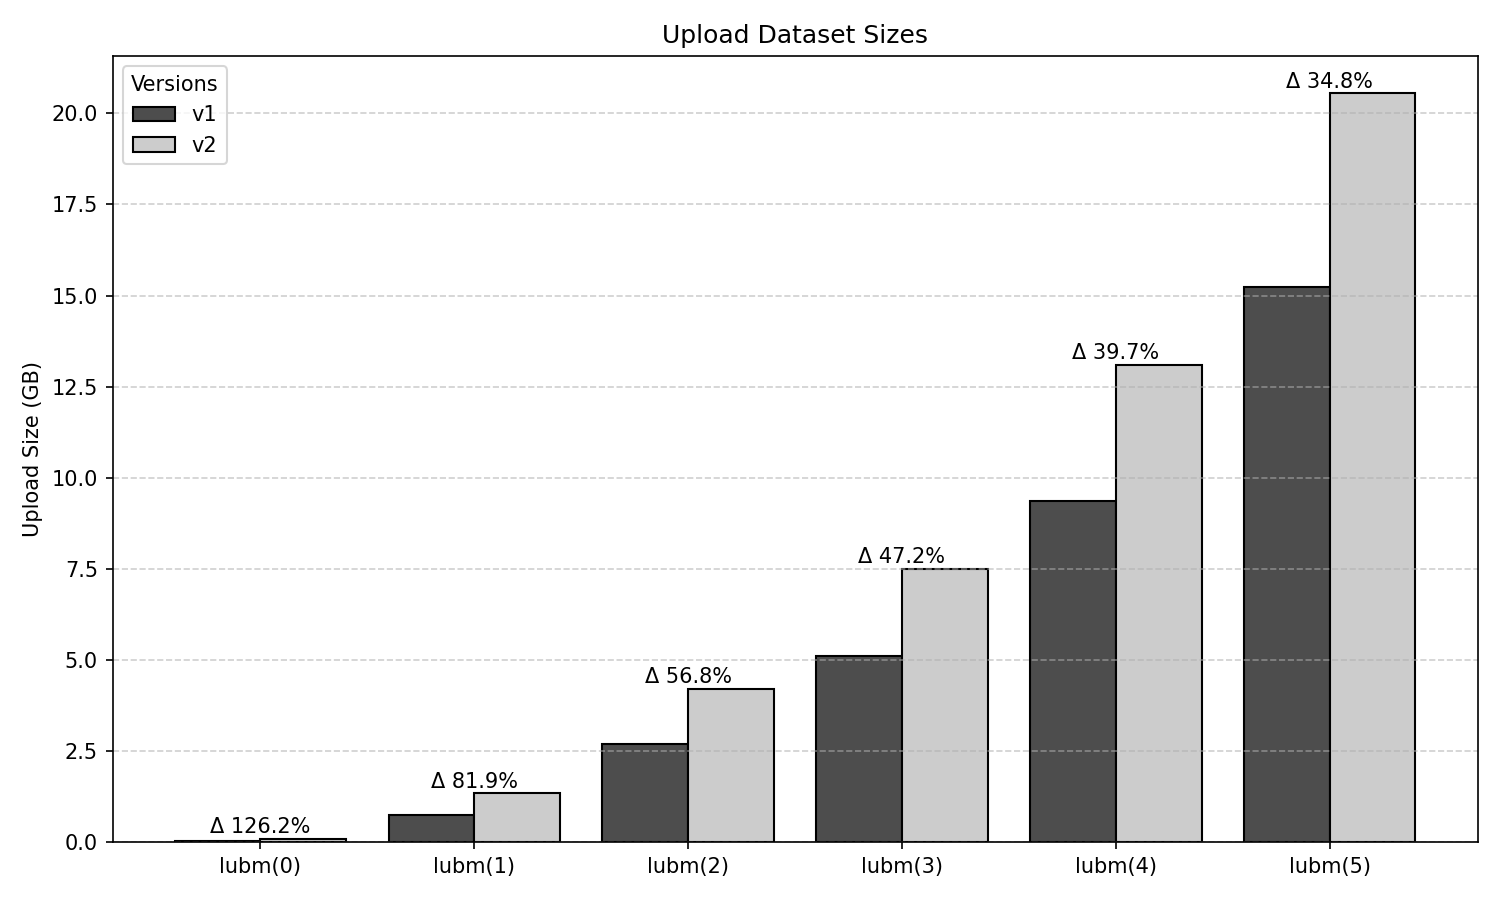
\includegraphics[width=\linewidth]{Figures/chapter5/lubm/upload_dataset_sizes.png}
    \caption{Dataset size, after upload.}
    \label{plot:upload-size}
\end{figure}

\begin{figure}[H]
    \centering
    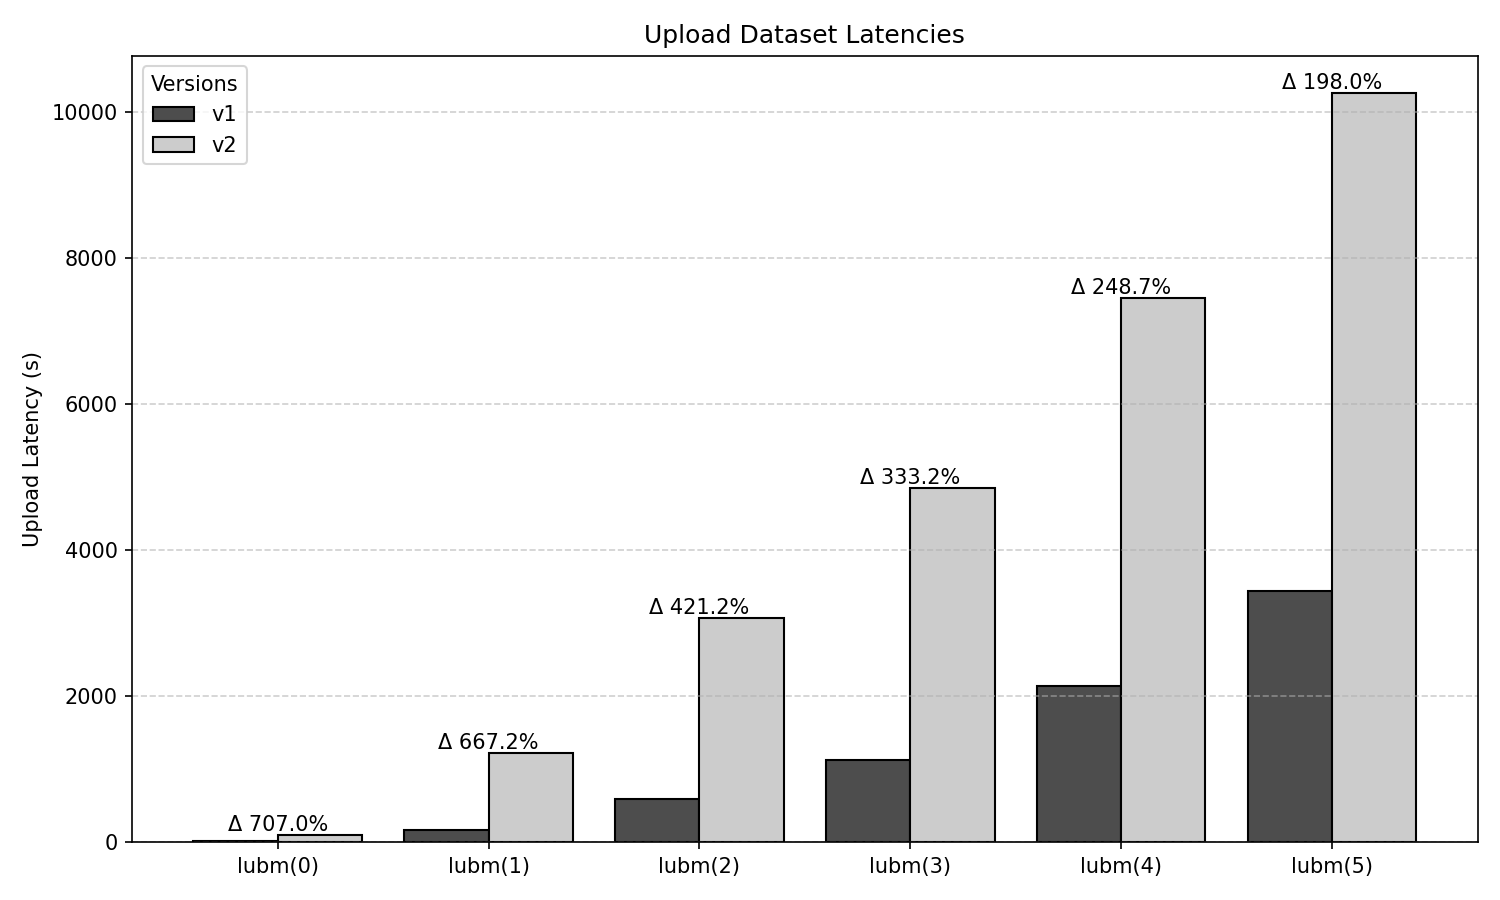
\includegraphics[width=\linewidth]{Figures/chapter5/lubm/upload_dataset_latency.png}
    \caption{Dataset upload latency.}
    \label{plot:upload-latency}
\end{figure}

\begin{figure}[H]
    \centering
    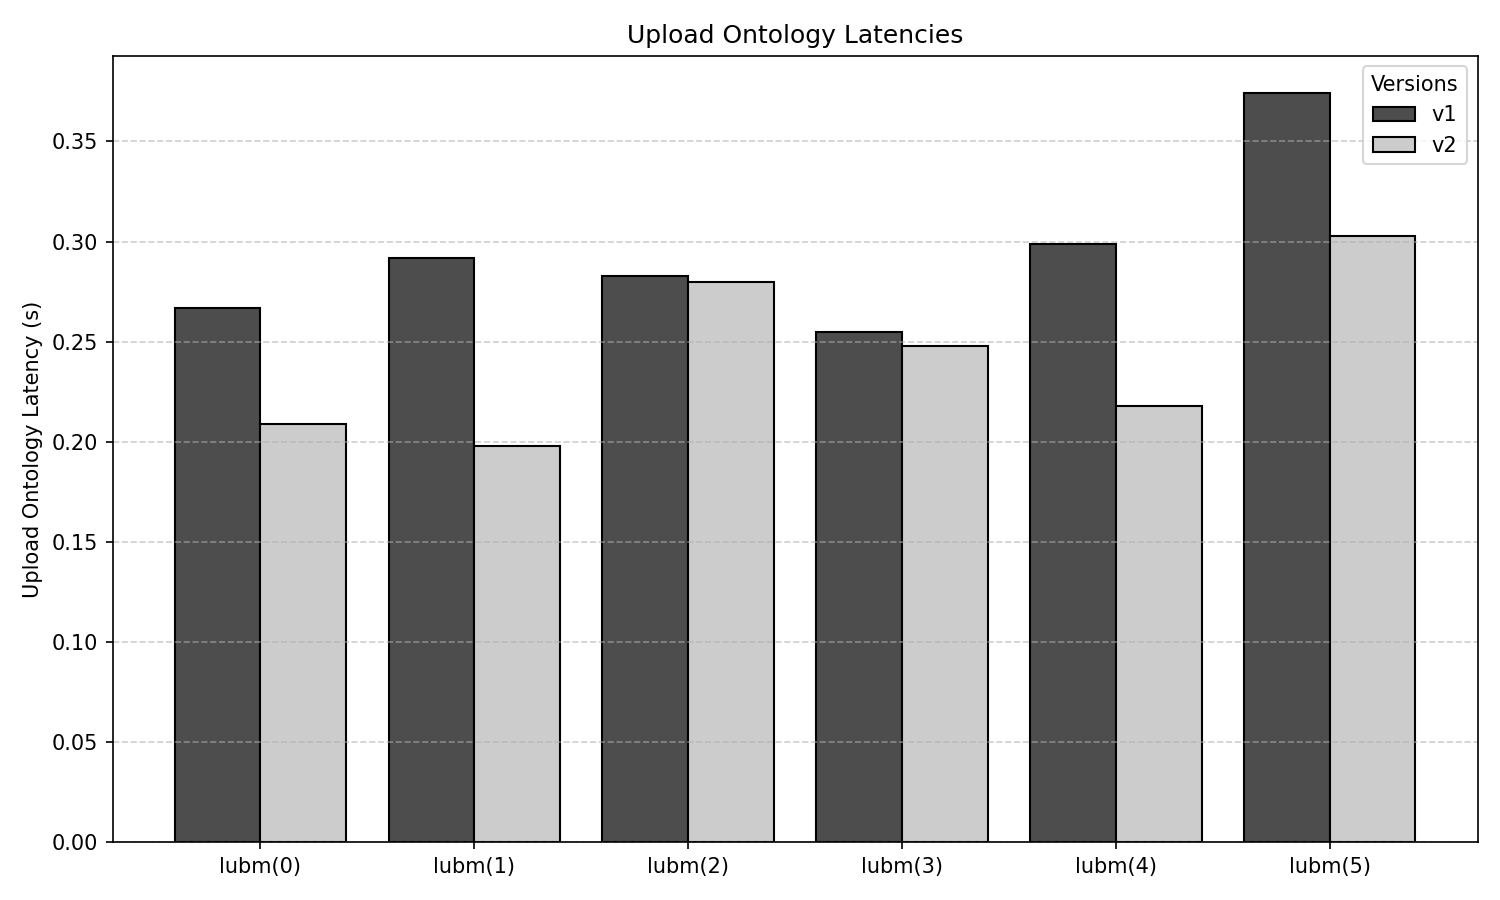
\includegraphics[width=\linewidth]{Figures/chapter5/lubm/upload_ontology_latency.png}
    \caption{Ontology upload latency.}
    \label{plot:upload-ontology-latency}
\end{figure}

\begin{figure}[H]
    \centering
    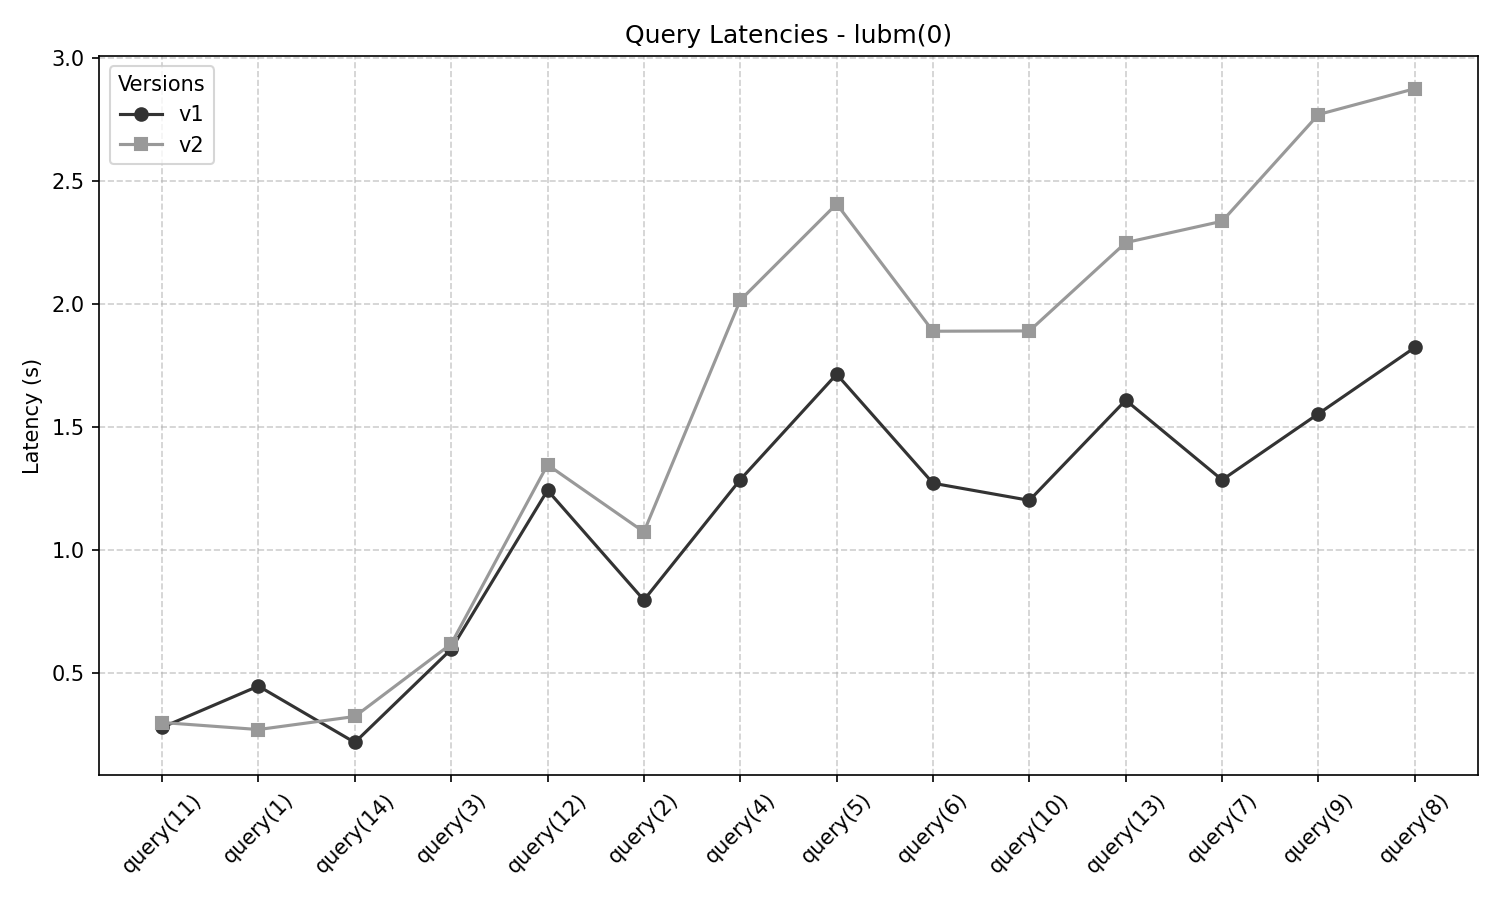
\includegraphics[width=\linewidth]{Figures/chapter5/lubm/latency_lubm-0.png}
    \caption{Query response latency for lubm(0).}
    \label{plot-latency-0}
\end{figure}

\begin{figure}[H]
    \centering
    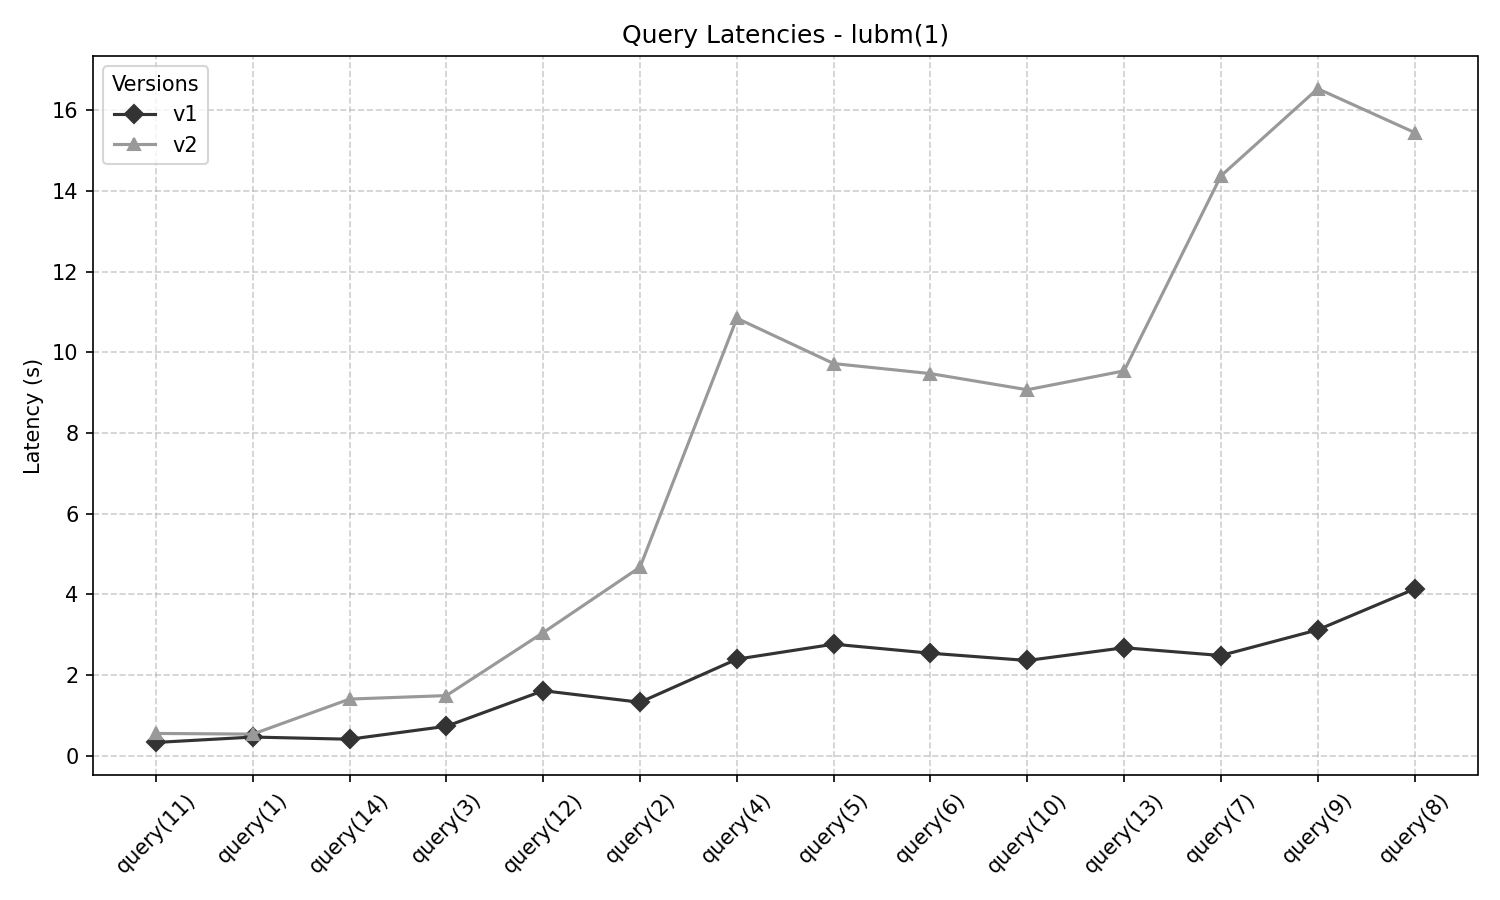
\includegraphics[width=\linewidth]{Figures/chapter5/lubm/latency_lubm-1.png}
    \caption{Query response latency for lubm(1).}
    \label{plot-latency-1}
\end{figure}

\begin{figure}[H]
    \centering
    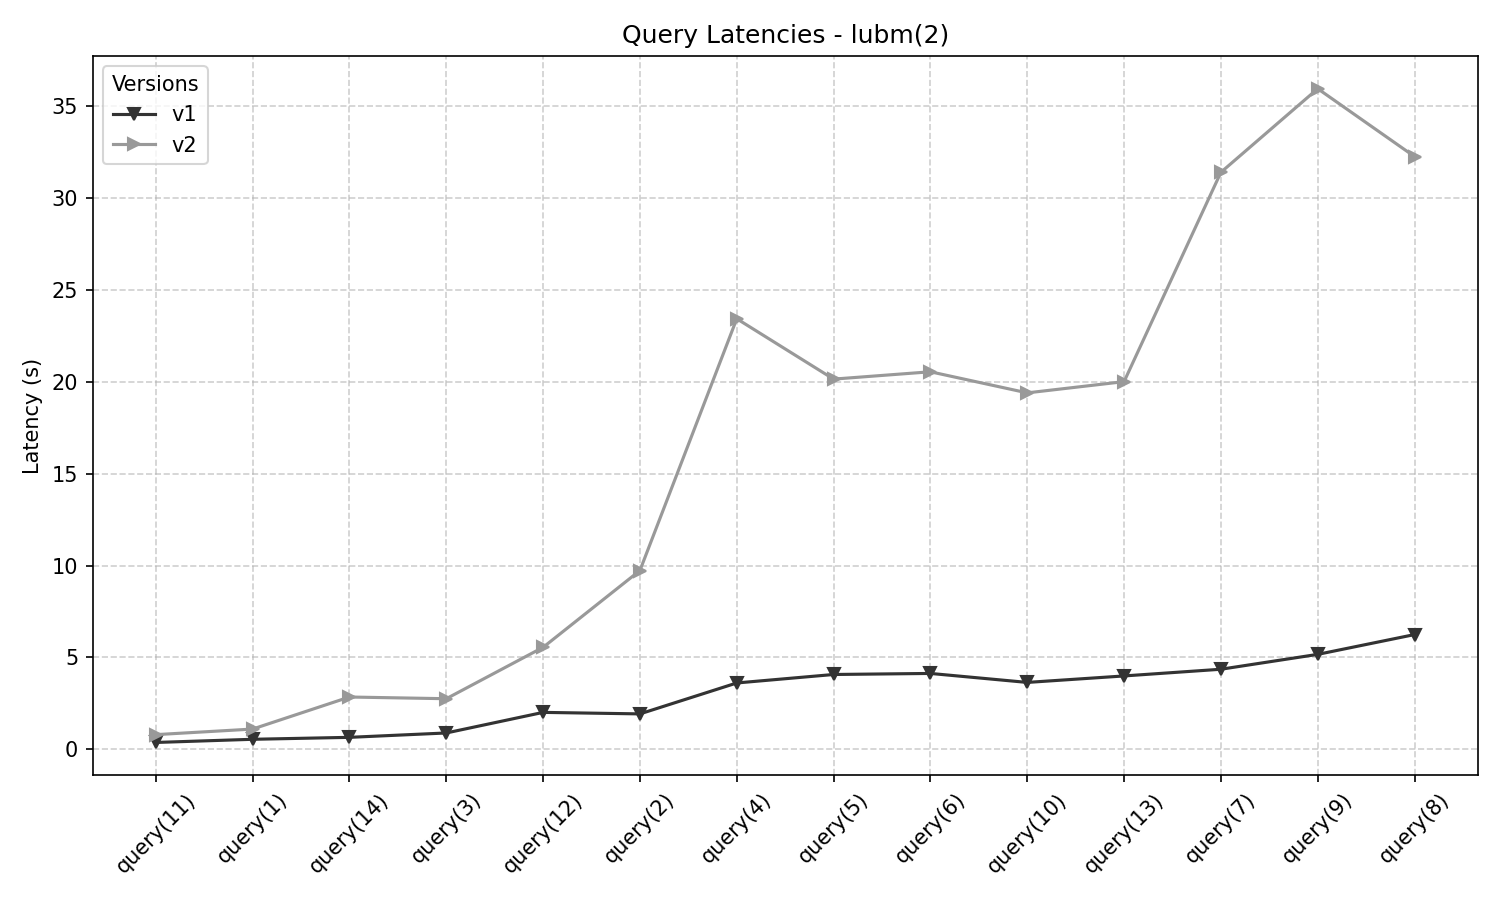
\includegraphics[width=\linewidth]{Figures/chapter5/lubm/latency_lubm-2.png}
    \caption{Query response latency for lubm(2).}
    \label{plot-latency-2}
\end{figure}

\begin{figure}[H]
    \centering
    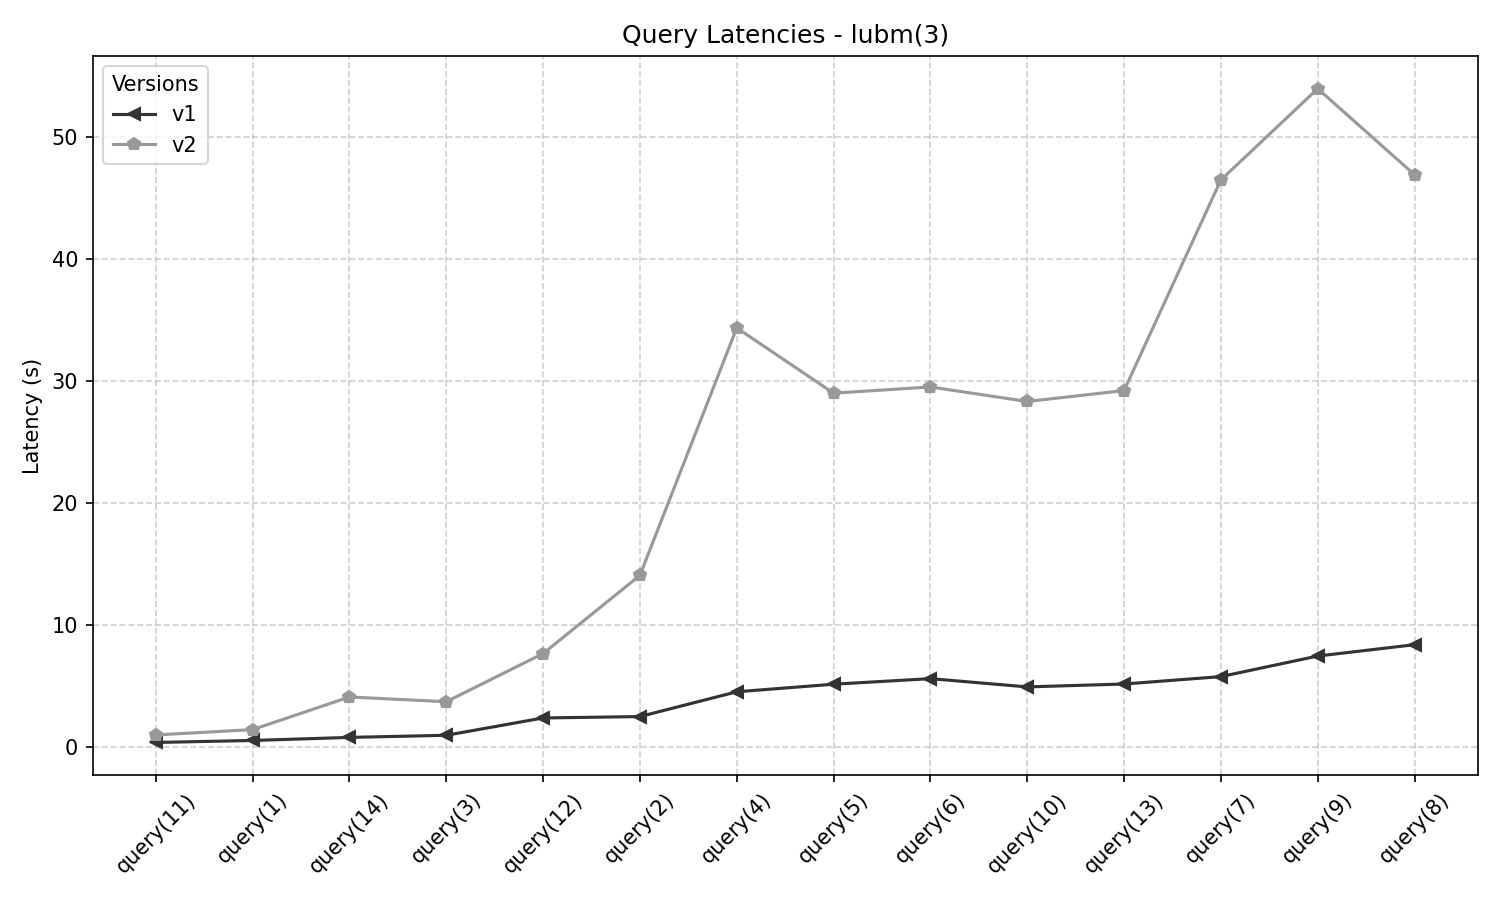
\includegraphics[width=\linewidth]{Figures/chapter5/lubm/latency_lubm-3.png}
    \caption{Query response latency for lubm(3).}
    \label{plot-latency-3}
\end{figure}

\begin{figure}[H]
    \centering
    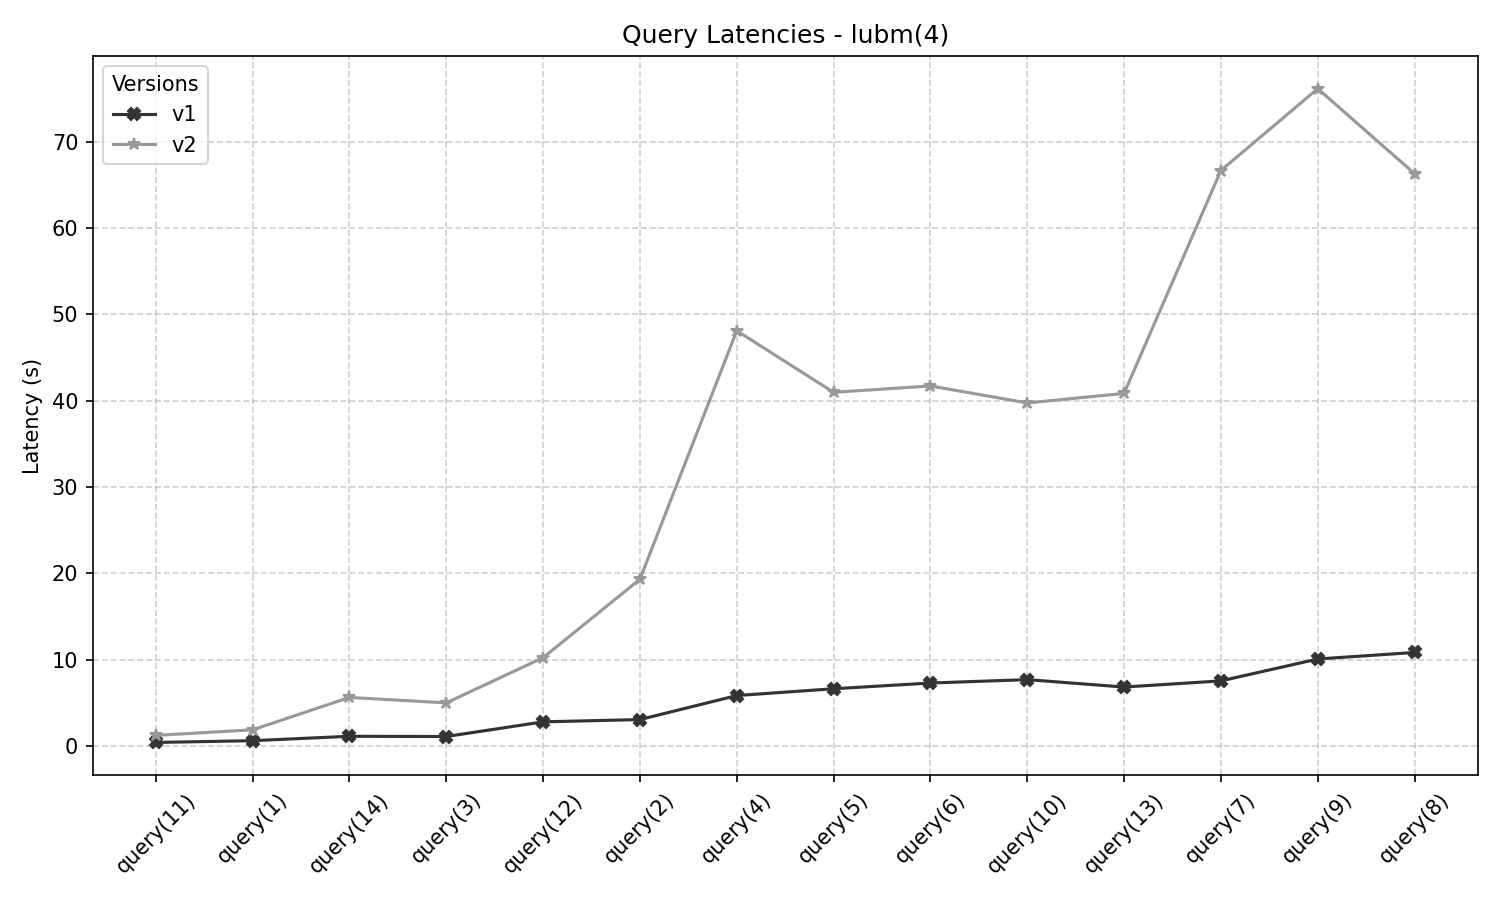
\includegraphics[width=\linewidth]{Figures/chapter5/lubm/latency_lubm-4.png}
    \caption{Query response latency for lubm(4).}
    \label{plot-latency-4}
\end{figure}

\begin{figure}[H]
    \centering
    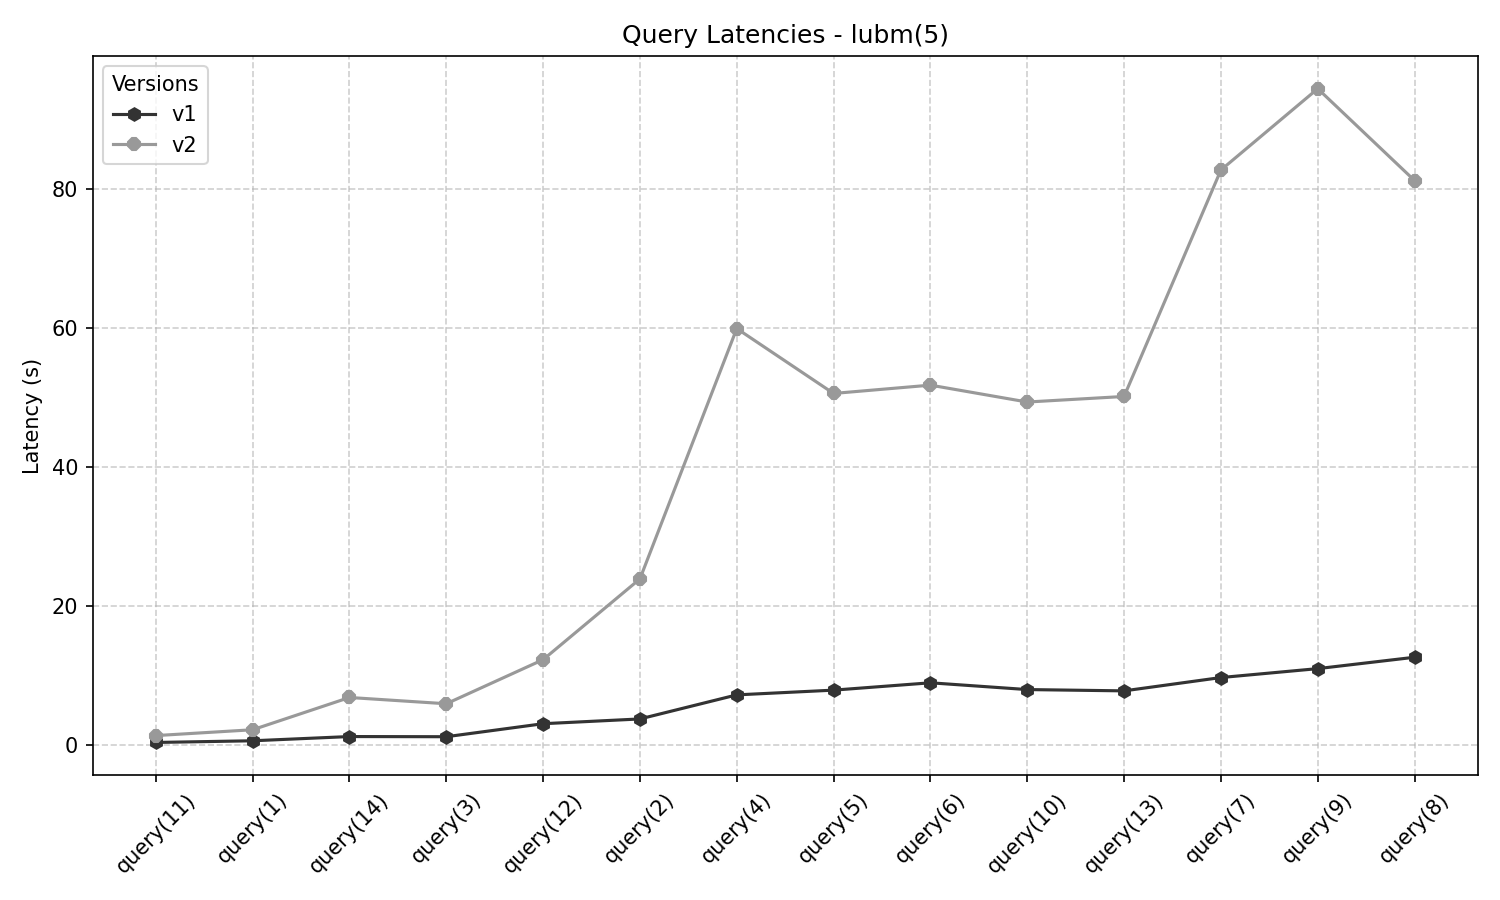
\includegraphics[width=\linewidth]{Figures/chapter5/lubm/latency_lubm-5.png}
    \caption{Query response latency for lubm(5).}
    \label{plot-latency-5}
\end{figure}

\begin{figure}[H]
    \centering
    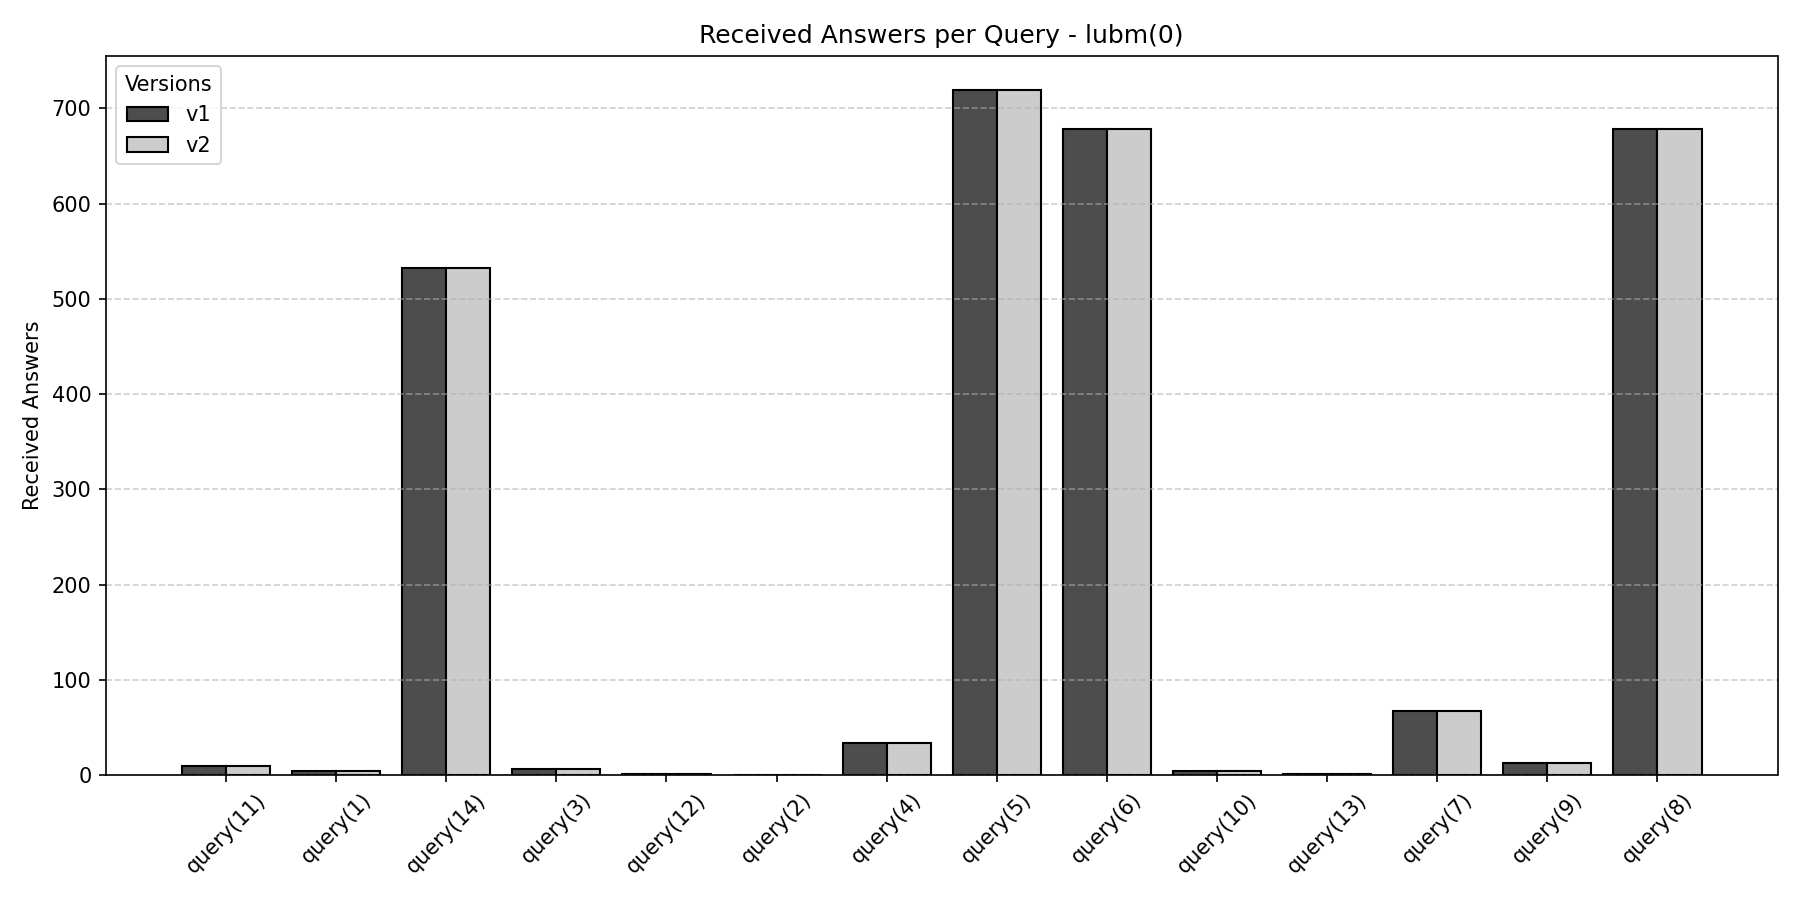
\includegraphics[width=\linewidth]{Figures/chapter5/lubm/received_answers_lubm-0.png}
    \caption{Received answers for lubm(0).}
    \label{plot-query-results-0}
\end{figure}

\begin{figure}[H]
    \centering
    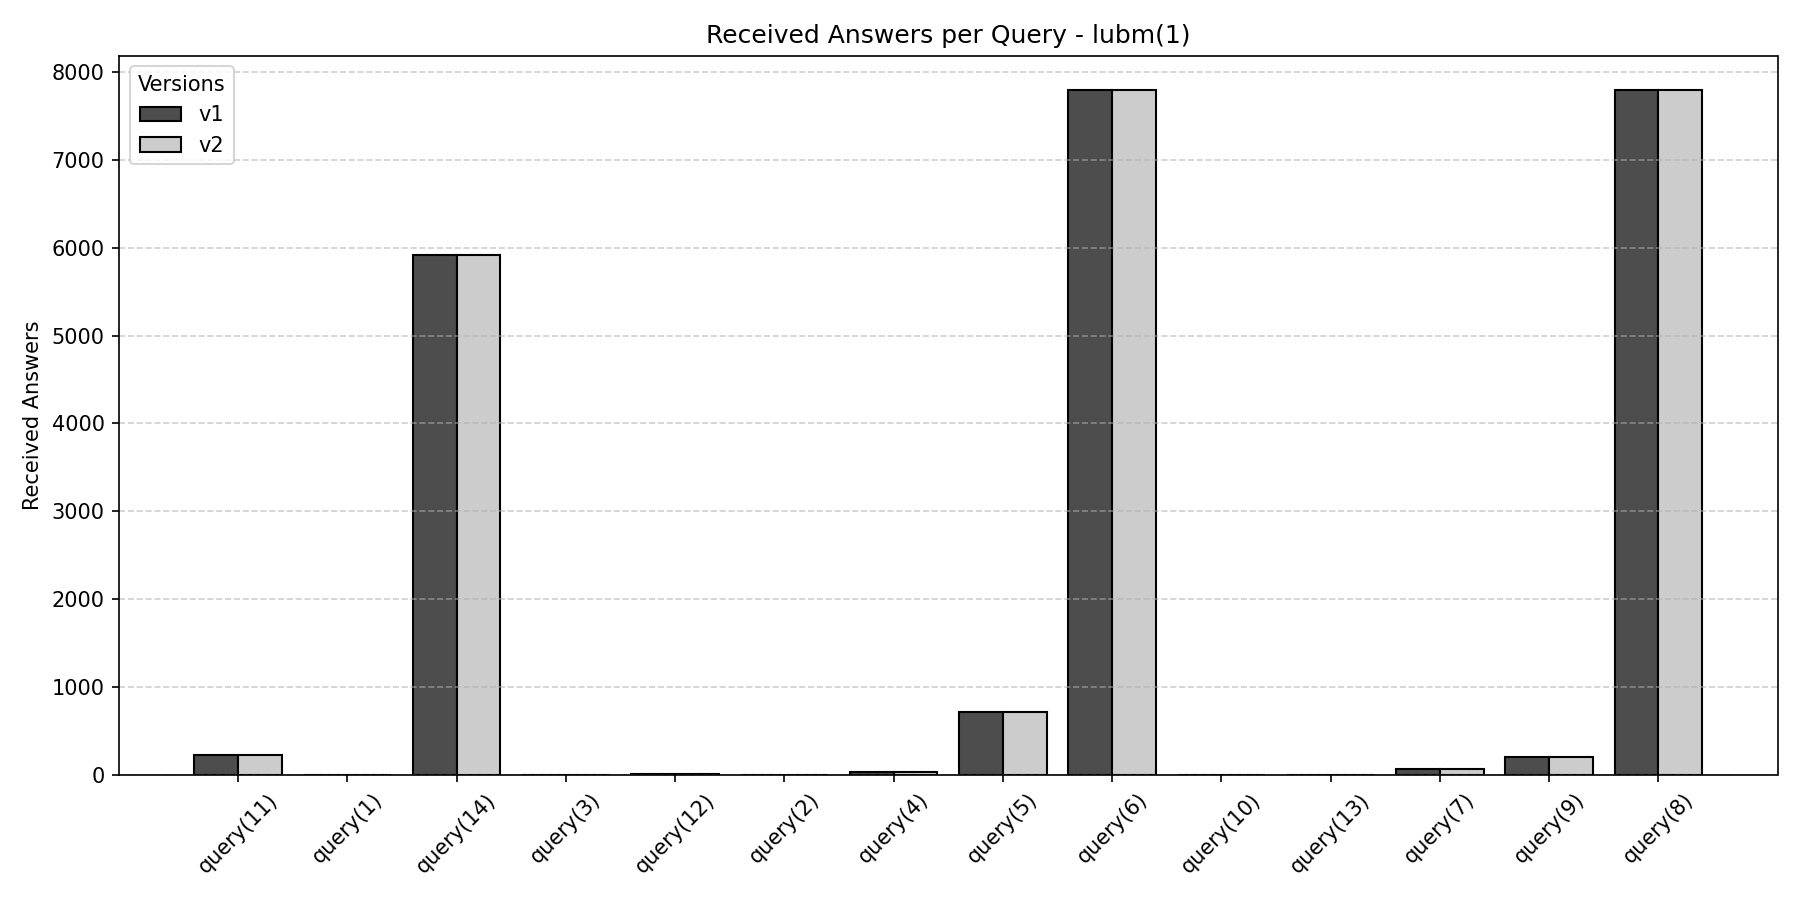
\includegraphics[width=\linewidth]{Figures/chapter5/lubm/received_answers_lubm-1.png}
    \caption{Received answers for lubm(1).}
    \label{plot-query-results-1}
\end{figure}

\begin{figure}[H]
    \centering
    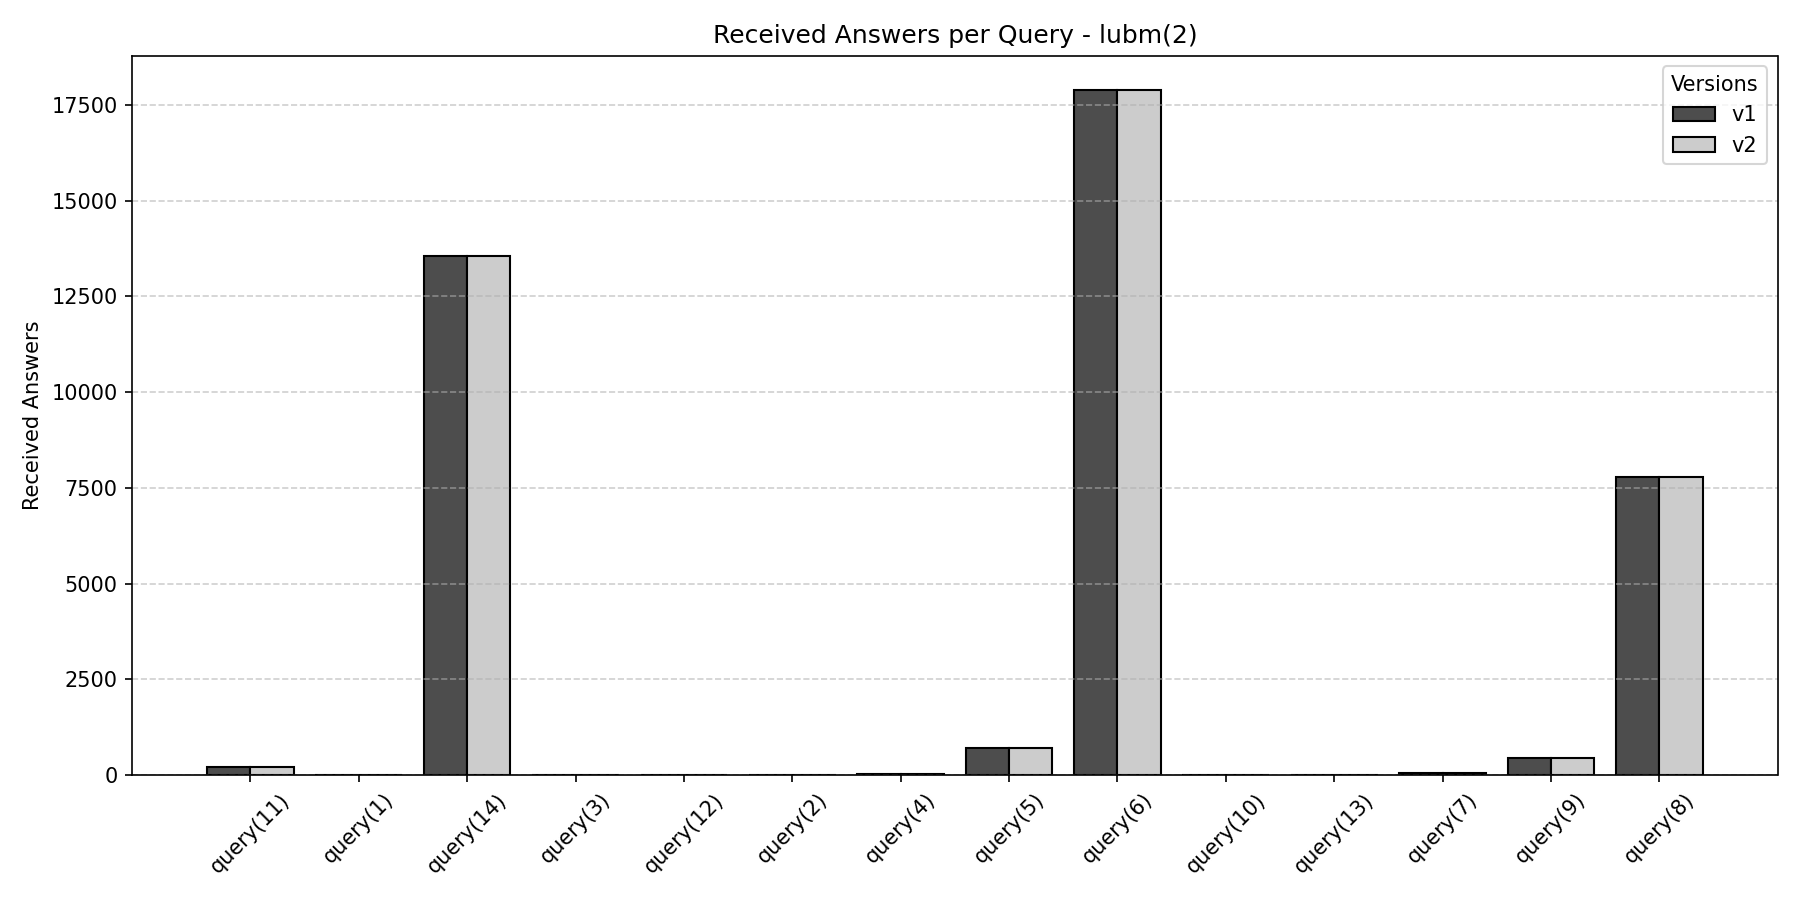
\includegraphics[width=\linewidth]{Figures/chapter5/lubm/received_answers_lubm-2.png}
    \caption{Received answers for lubm(2).}
    \label{plot-query-results-2}
\end{figure}

\begin{figure}[H]
    \centering
    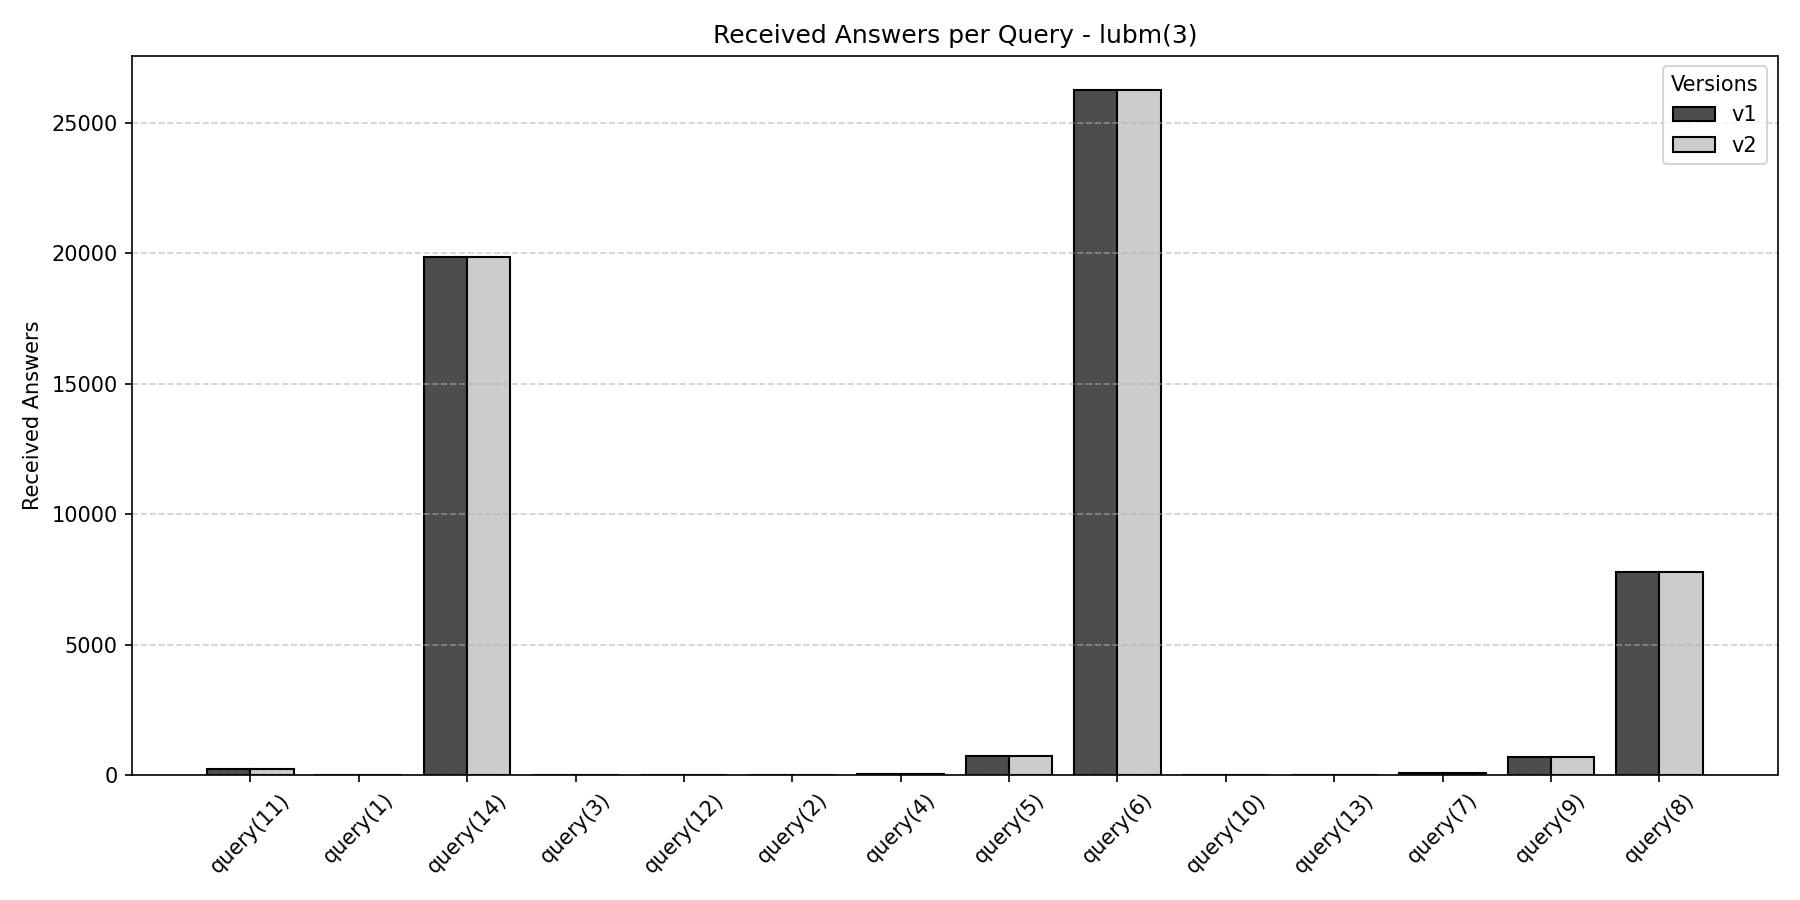
\includegraphics[width=\linewidth]{Figures/chapter5/lubm/received_answers_lubm-3.png}
    \caption{Received answers for lubm(3).}
    \label{plot-query-results-3}
\end{figure}

\begin{figure}[H]
    \centering
    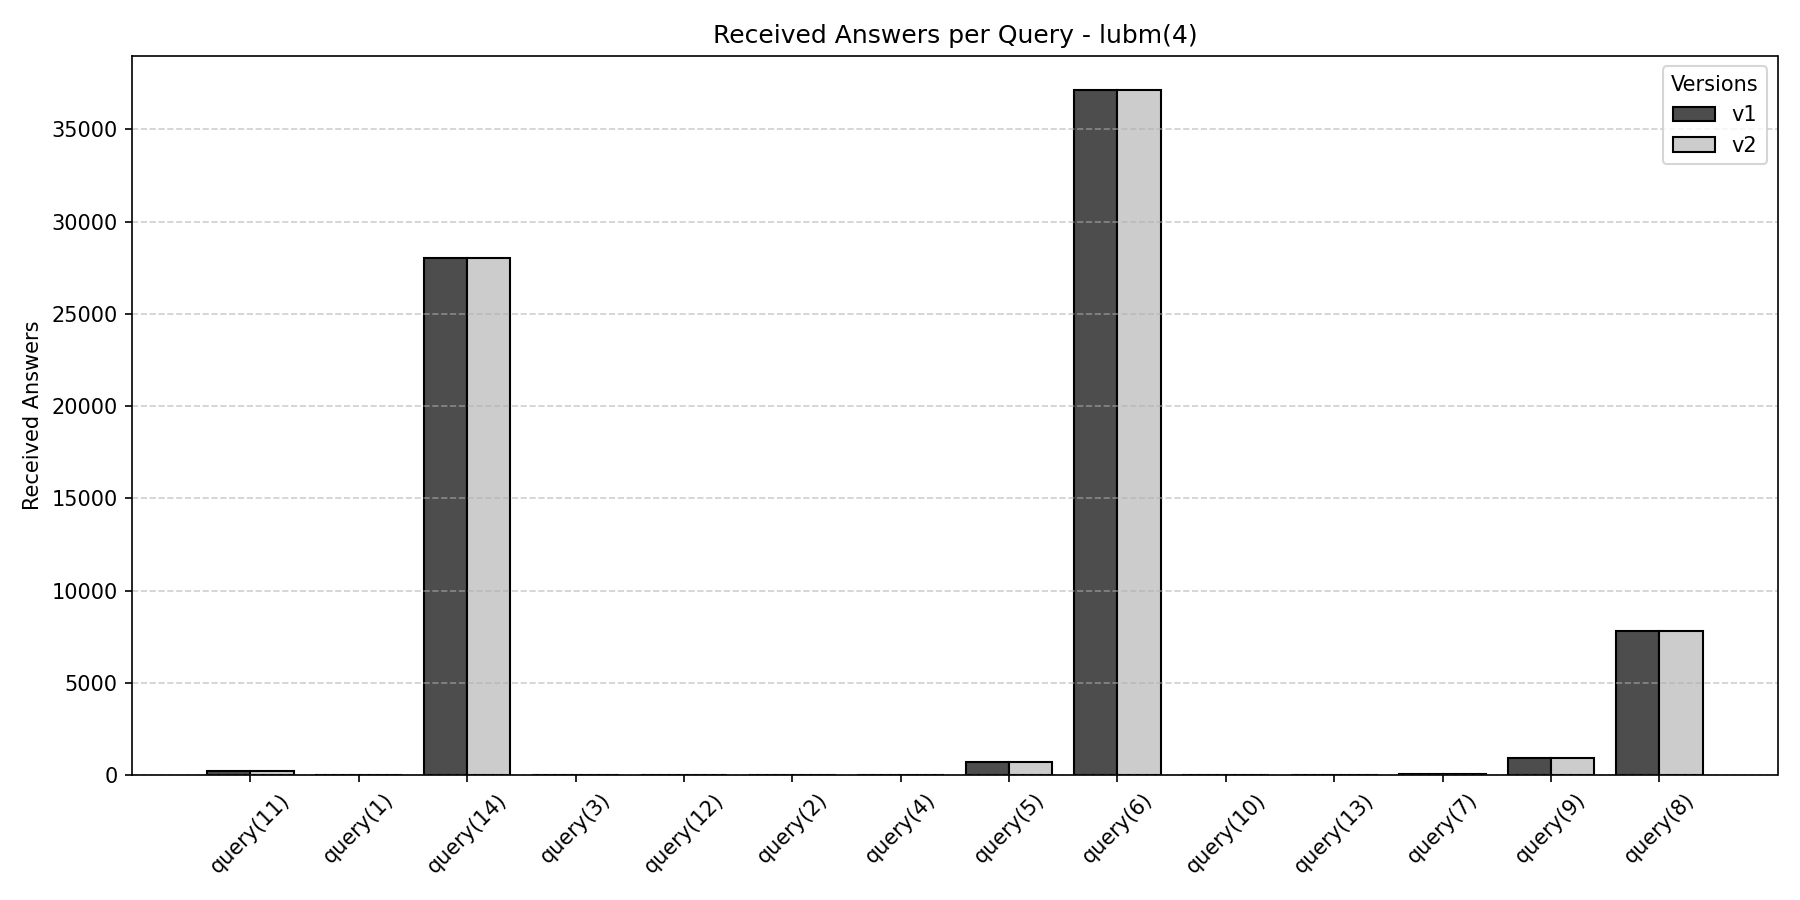
\includegraphics[width=\linewidth]{Figures/chapter5/lubm/received_answers_lubm-4.png}
    \caption{Received answers for lubm(4).}
    \label{plot-query-results-4}
\end{figure}

\begin{figure}[H]
    \centering
    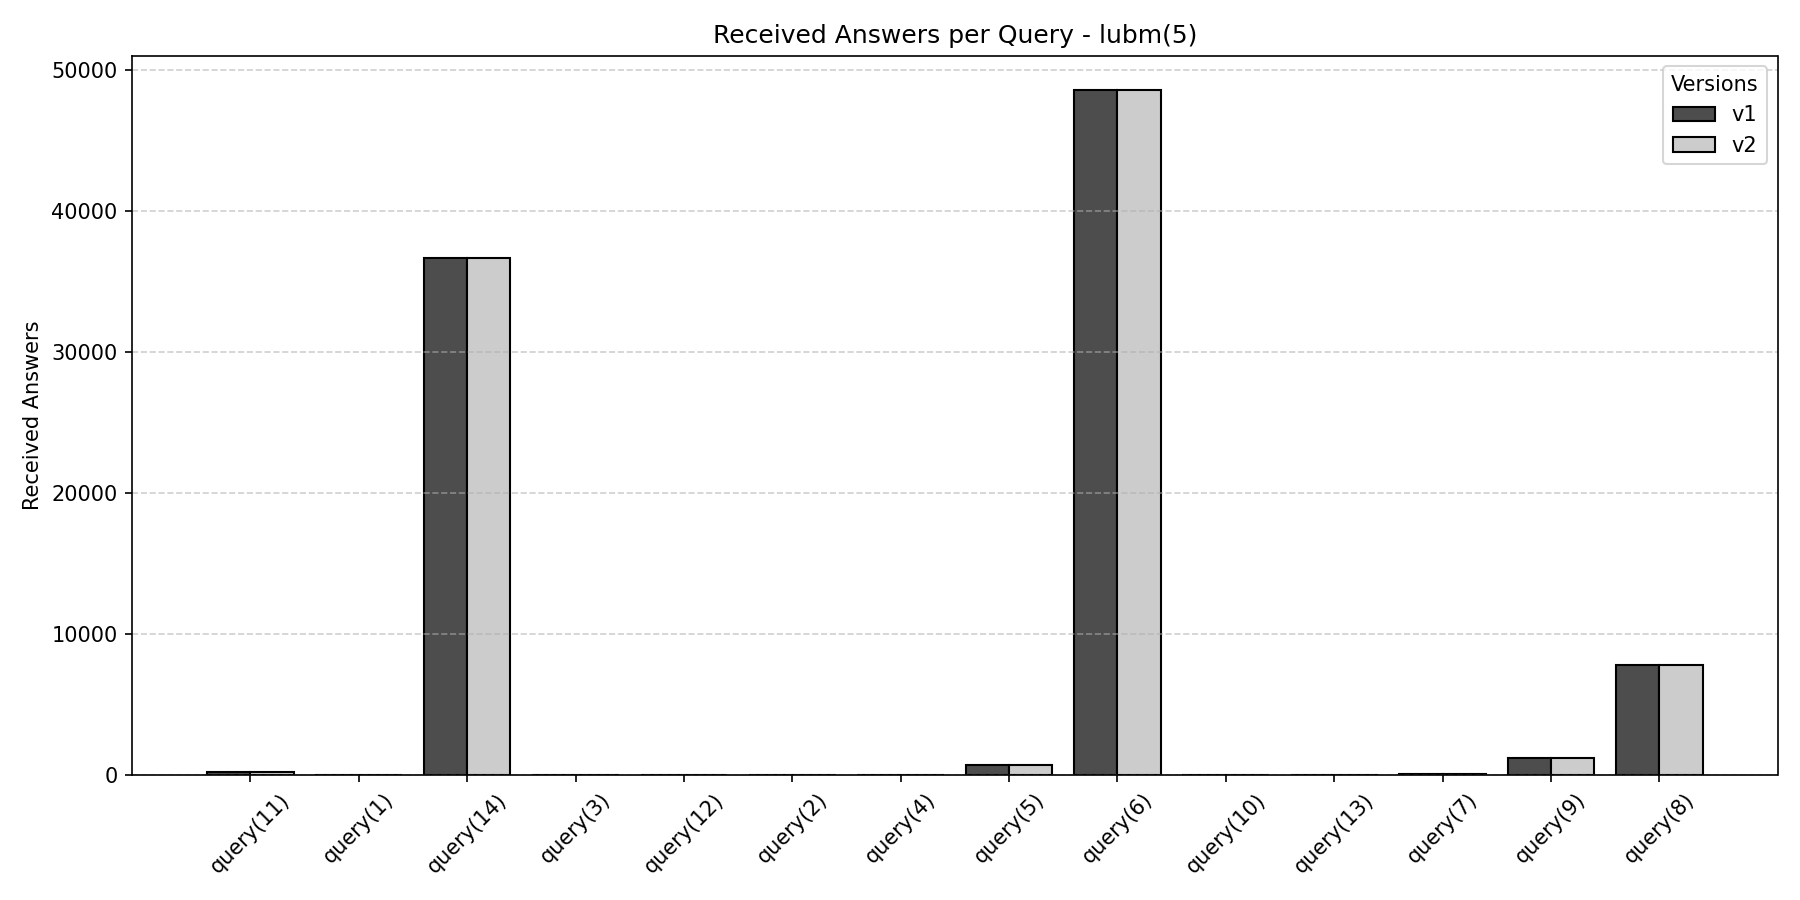
\includegraphics[width=\linewidth]{Figures/chapter5/lubm/received_answers_lubm-5.png}
    \caption{Received answers for lubm(5).}
    \label{plot-query-results-5}
\end{figure}

\begin{figure}[H]
    \centering
    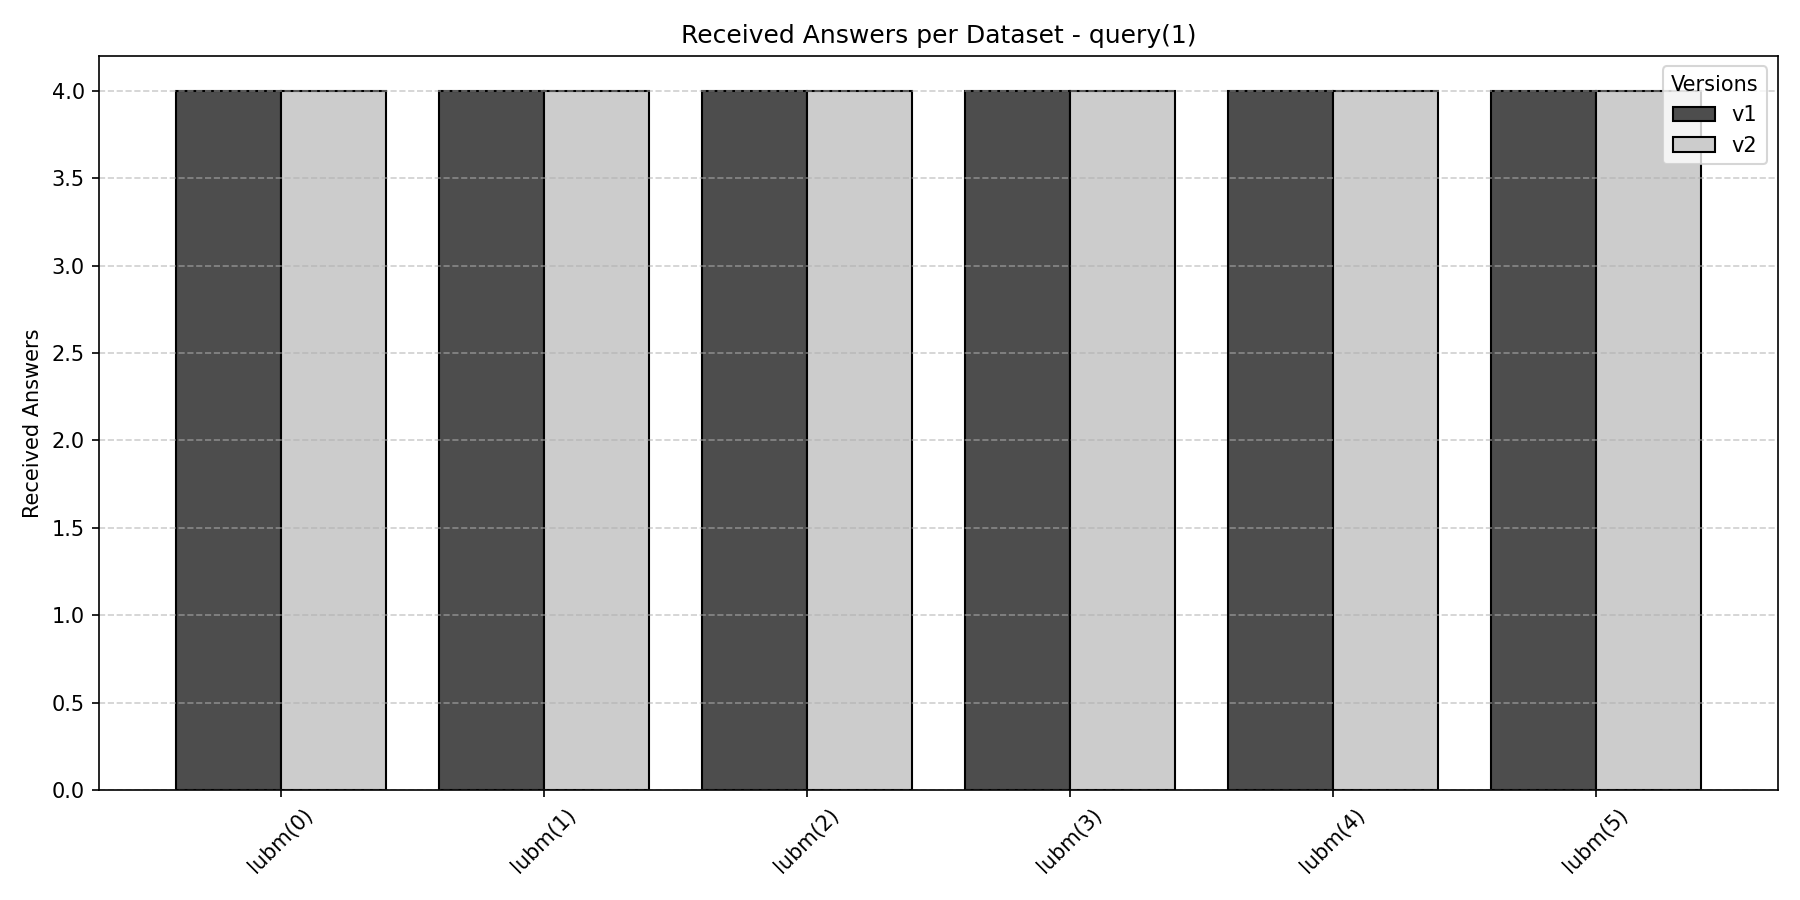
\includegraphics[width=\linewidth]{Figures/chapter5/lubm/received_answers_query1.png}
    \caption{Received answer for \gls{LUBM} query 1.}
    \label{plot-query-results-q1}
\end{figure}

\begin{figure}[H]
    \centering
    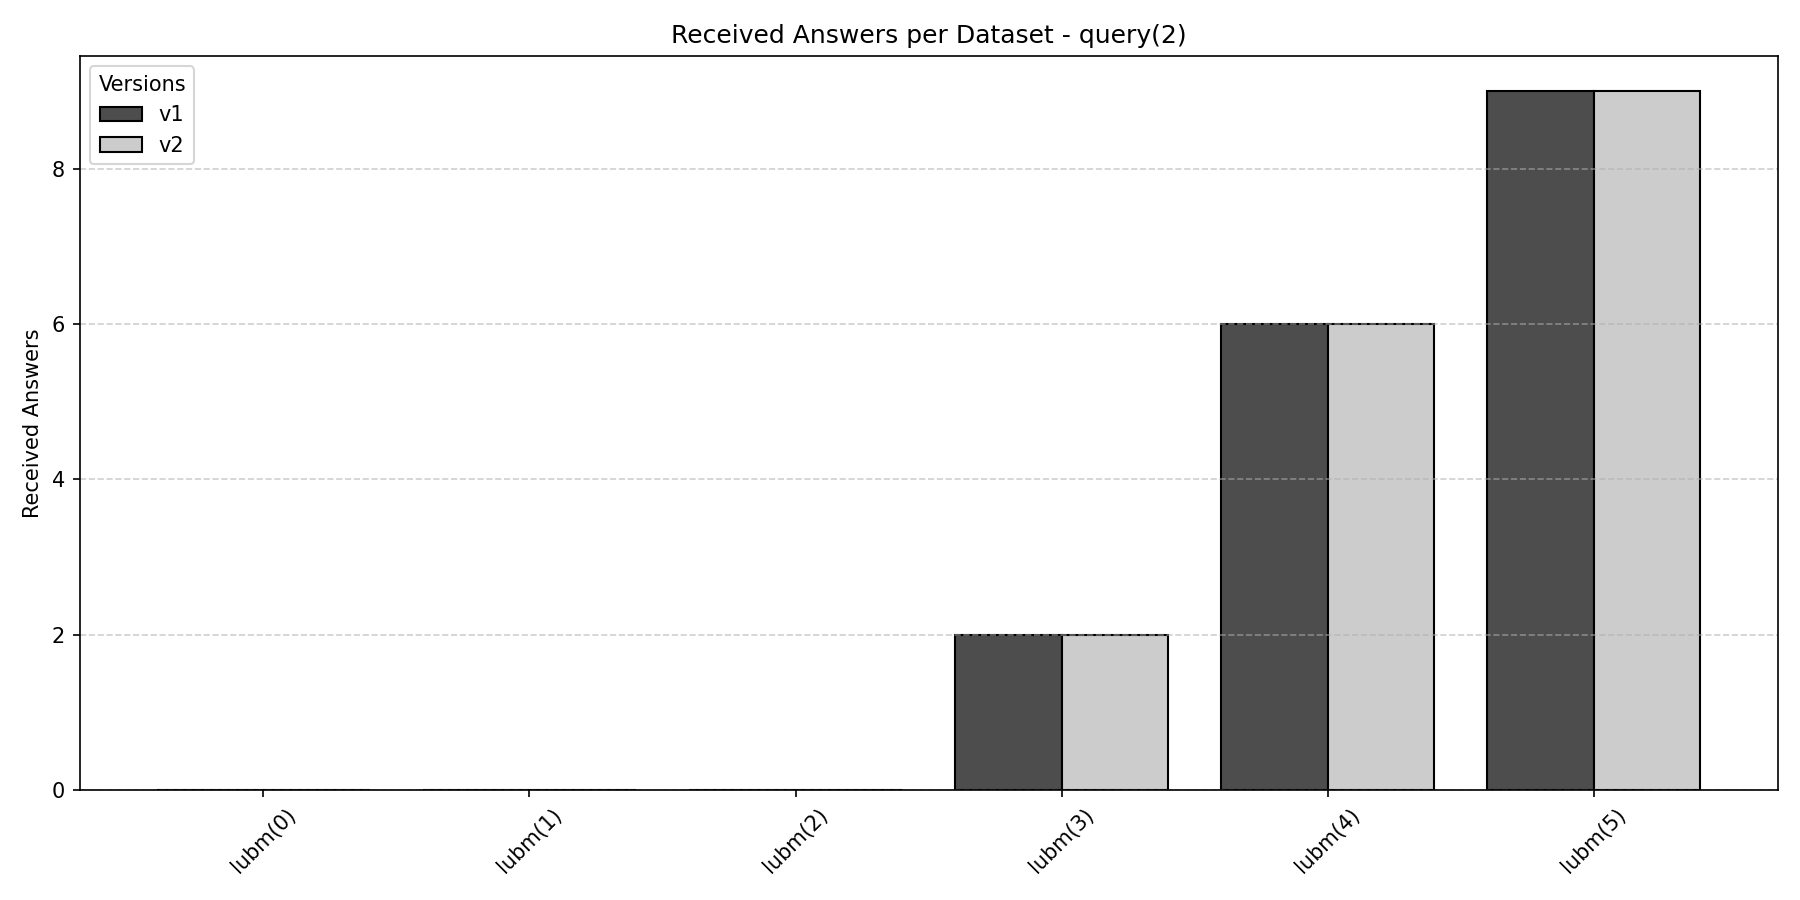
\includegraphics[width=\linewidth]{Figures/chapter5/lubm/received_answers_query2.png}
    \caption{Received answer for \gls{LUBM} query 2.}
    \label{plot-query-results-q2}
\end{figure}

\begin{figure}[H]
    \centering
    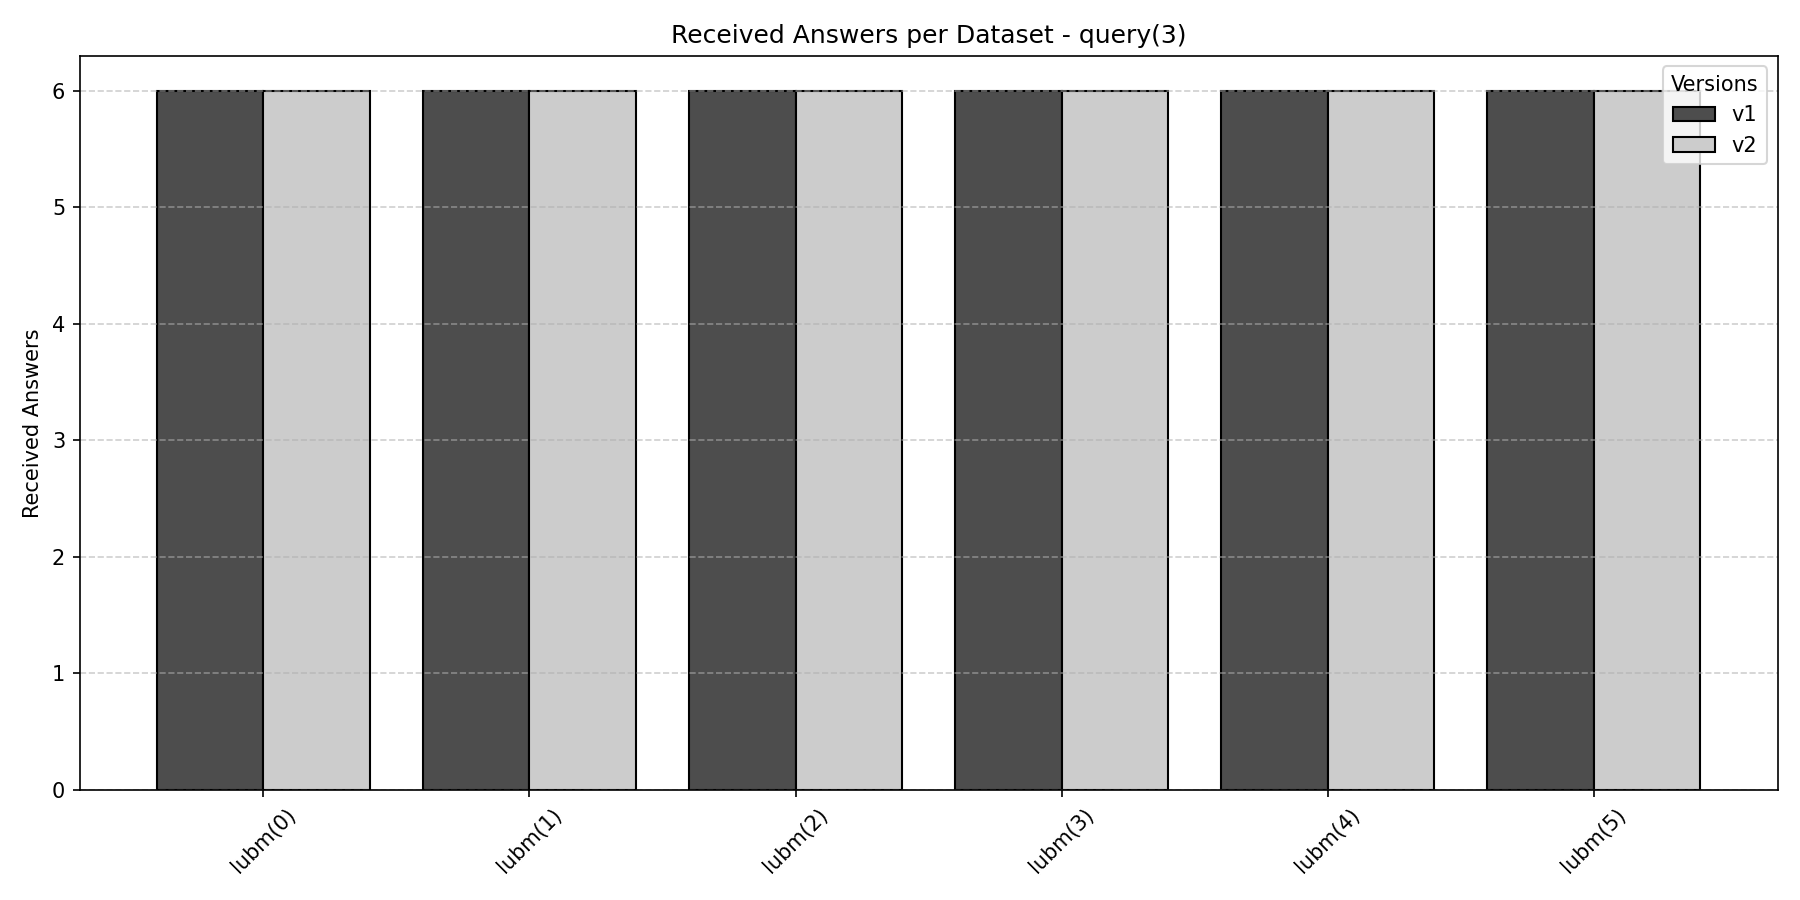
\includegraphics[width=\linewidth]{Figures/chapter5/lubm/received_answers_query3.png}
    \caption{Received answer for \gls{LUBM} query 3.}
    \label{plot-query-results-q3}
\end{figure}

\begin{figure}[H]
    \centering
    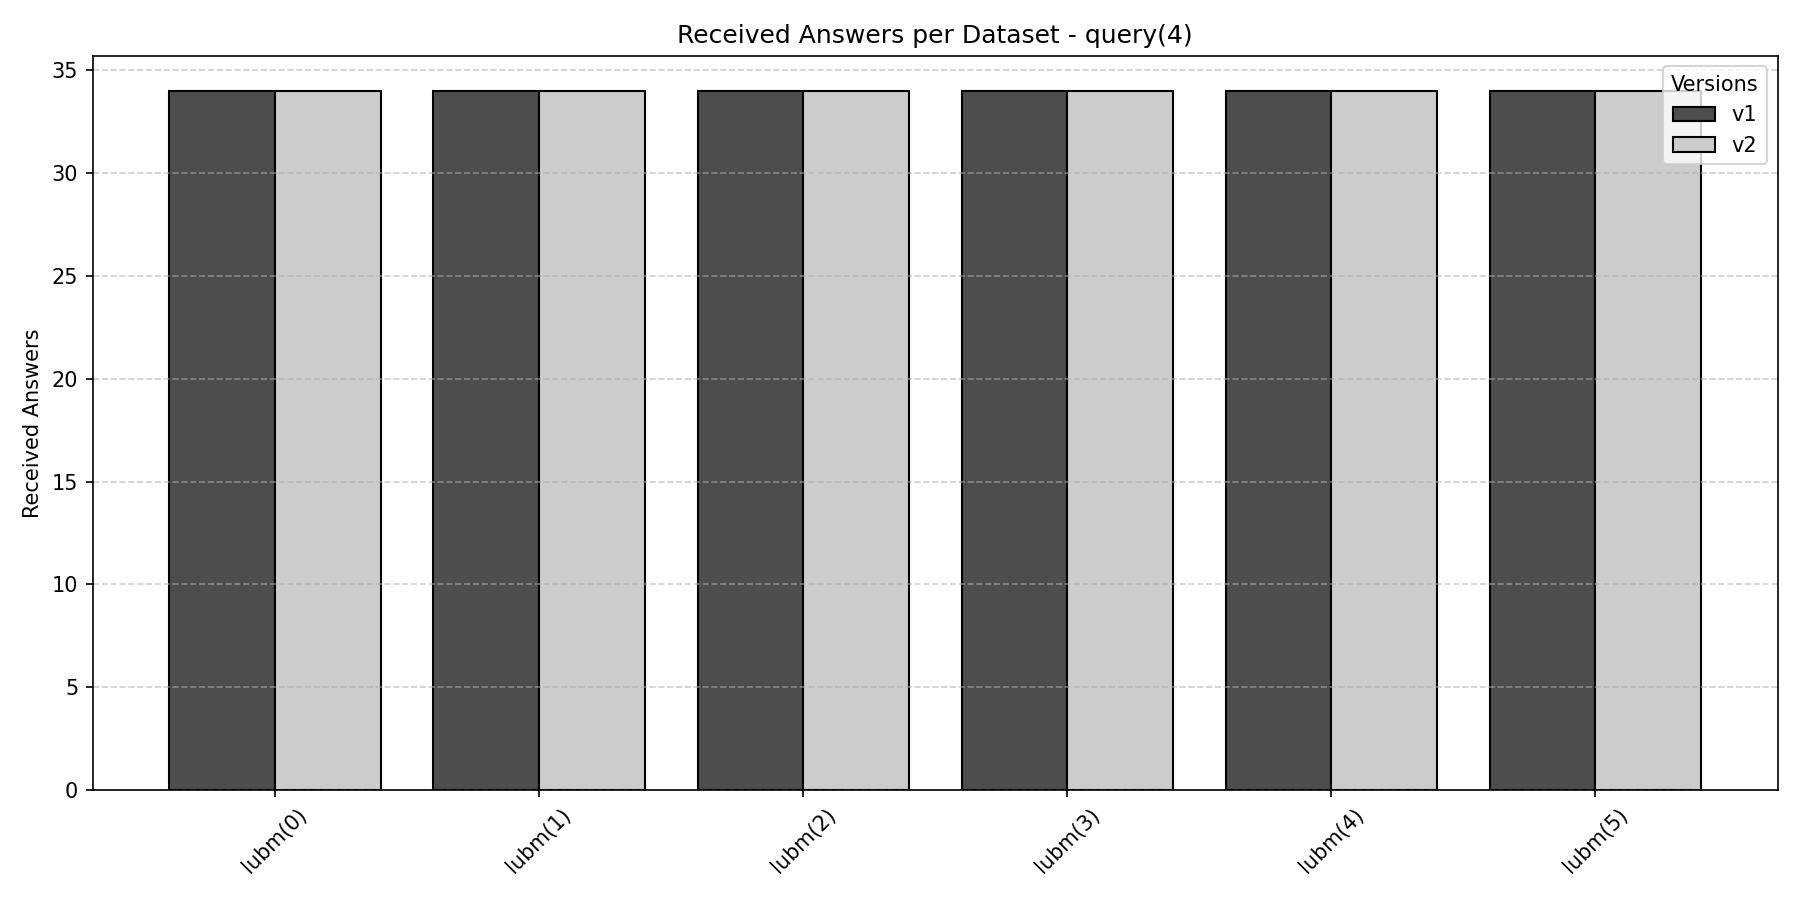
\includegraphics[width=\linewidth]{Figures/chapter5/lubm/received_answers_query4.png}
    \caption{Received answer for \gls{LUBM} query 4.}
    \label{plot-query-results-q4}
\end{figure}

\begin{figure}[H]
    \centering
    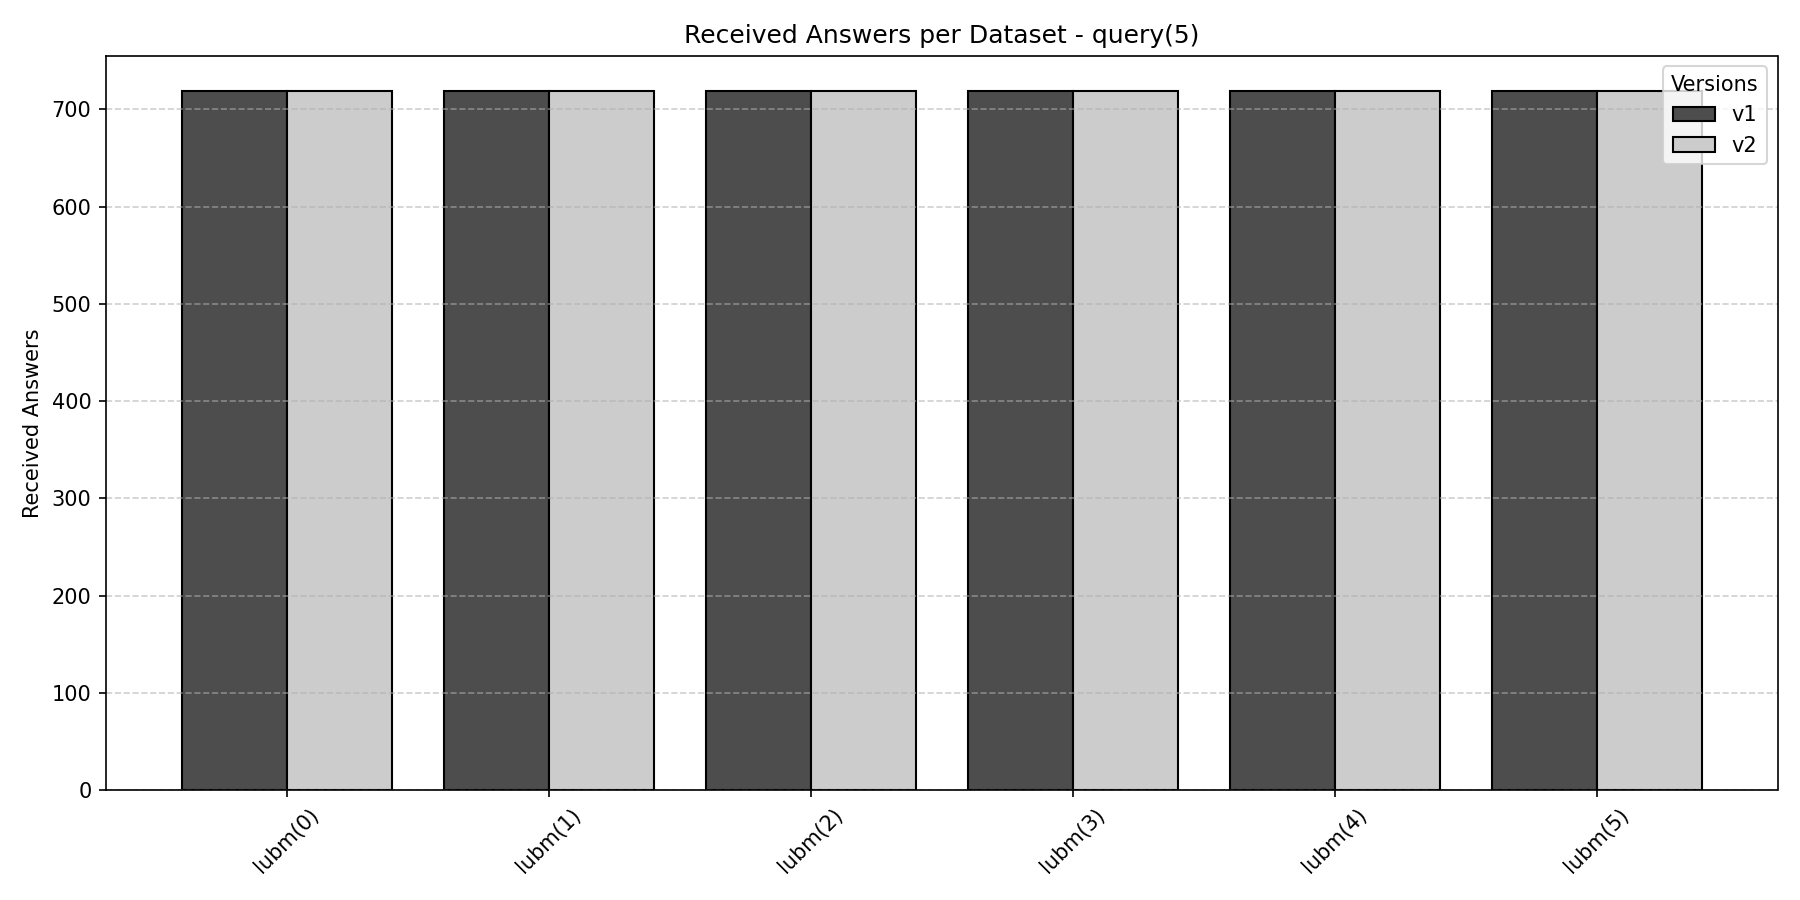
\includegraphics[width=\linewidth]{Figures/chapter5/lubm/received_answers_query5.png}
    \caption{Received answer for \gls{LUBM} query 5.}
    \label{plot-query-results-q5}
\end{figure}

\begin{figure}[H]
    \centering
    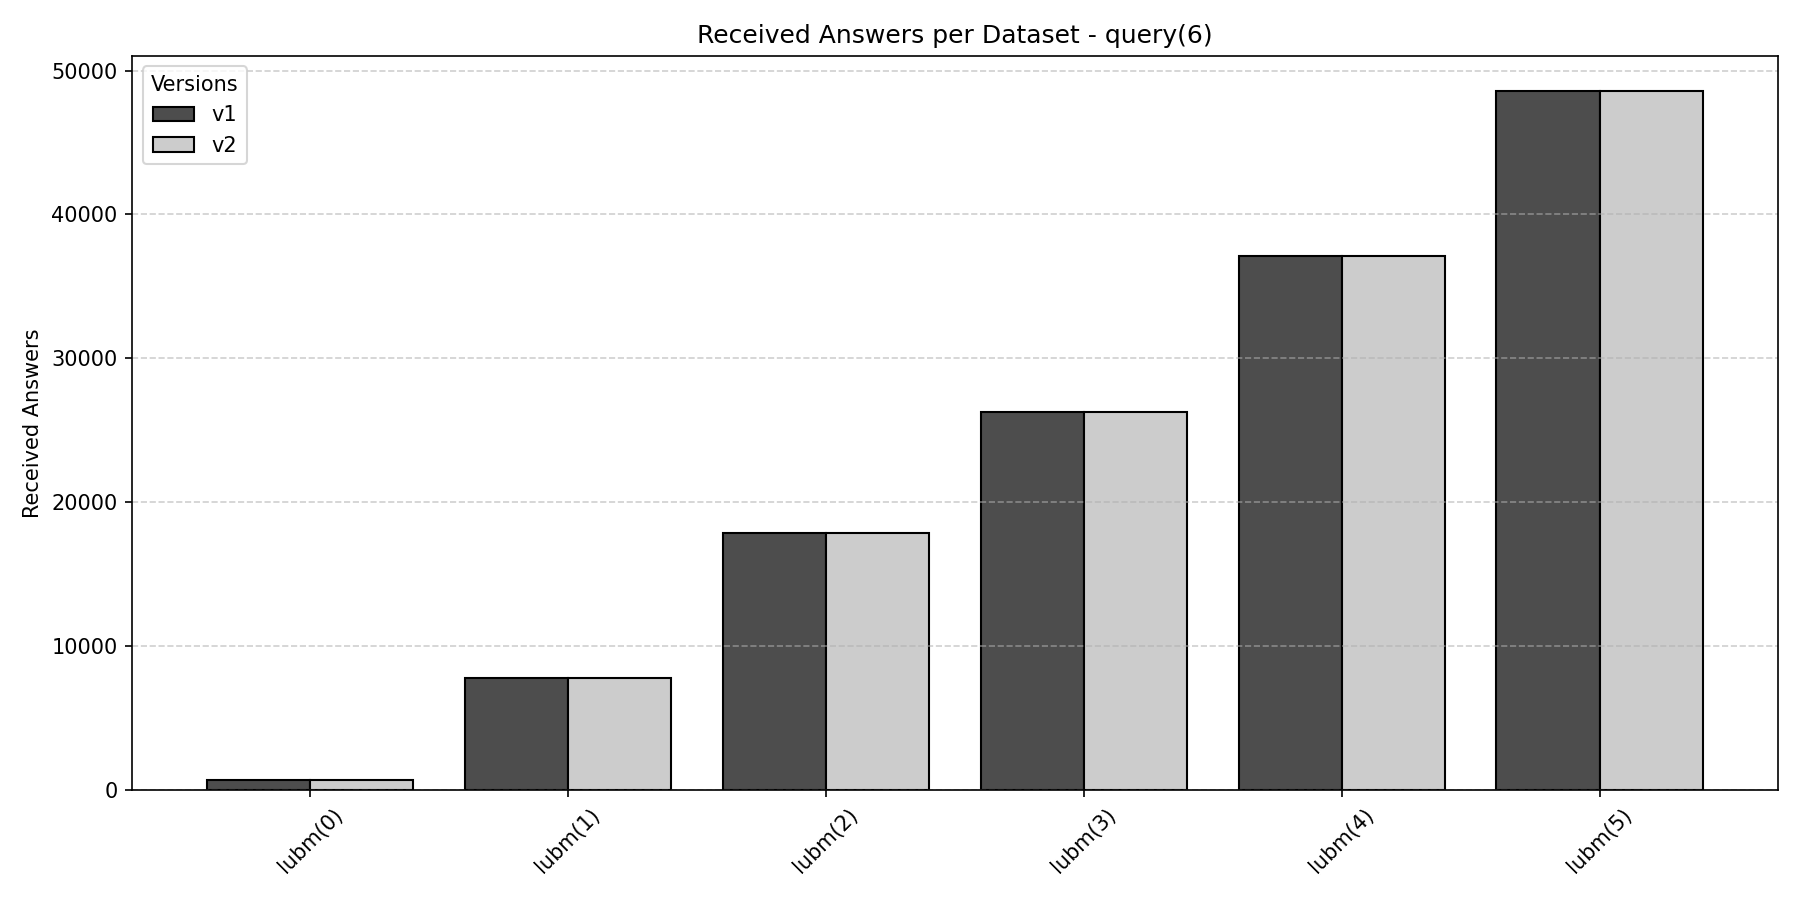
\includegraphics[width=\linewidth]{Figures/chapter5/lubm/received_answers_query6.png}
    \caption{Received answer for \gls{LUBM} query 6.}
    \label{plot-query-results-q6}
\end{figure}

\begin{figure}[H]
    \centering
    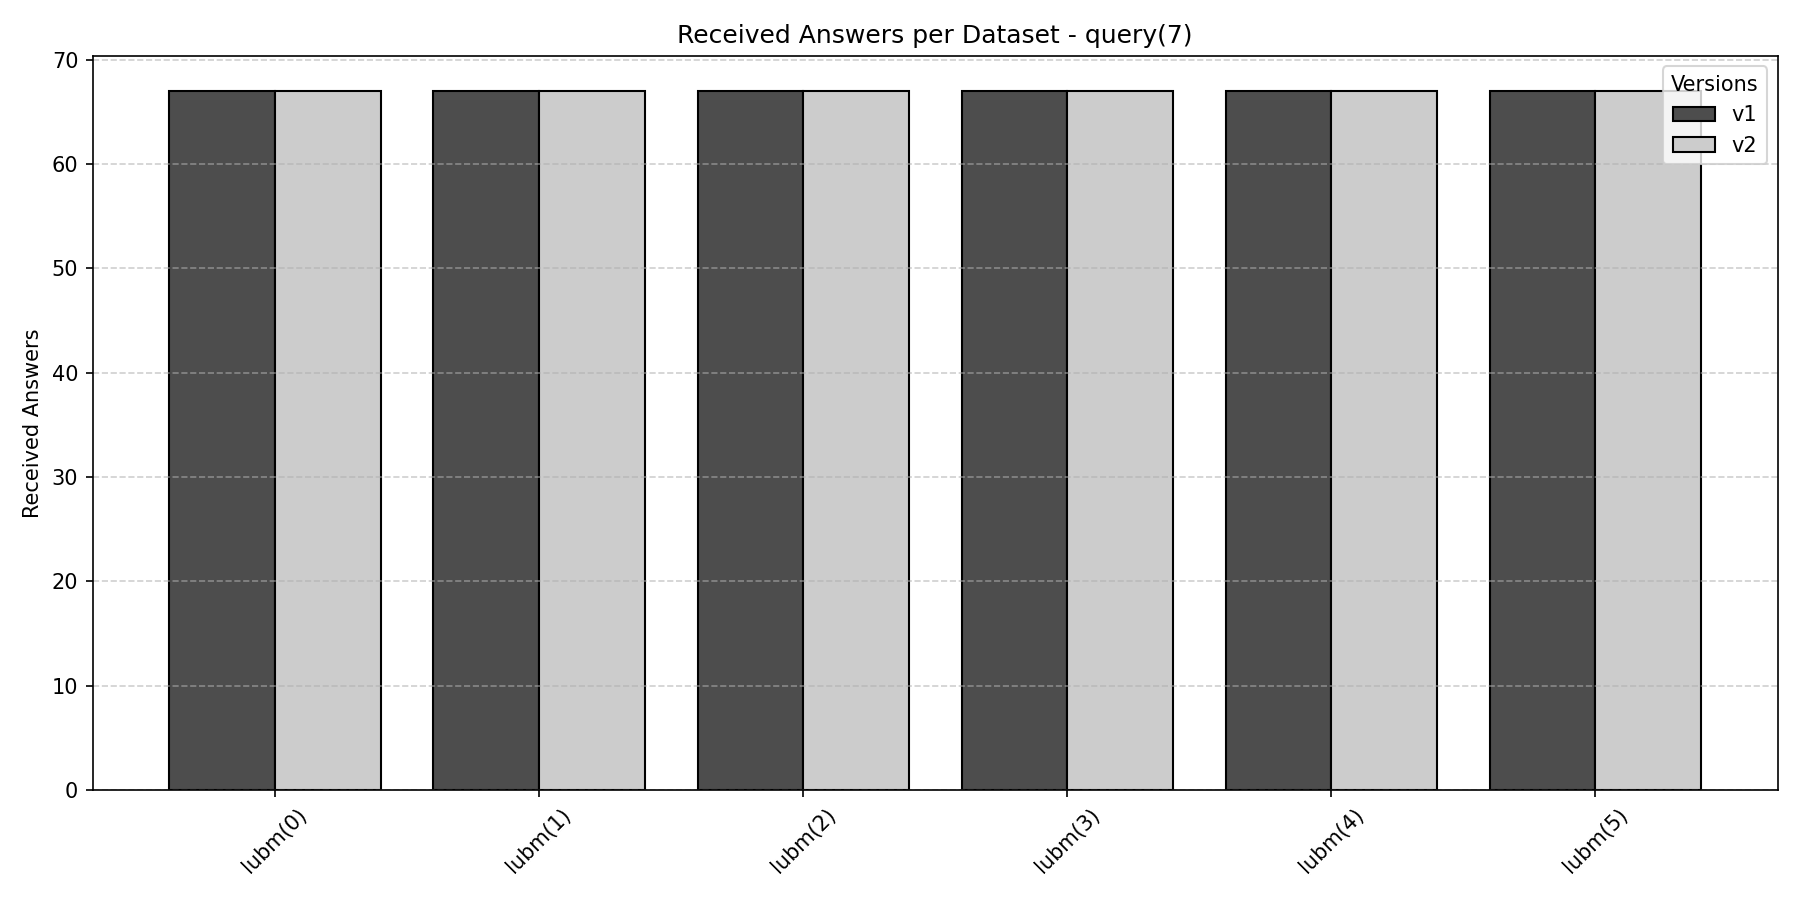
\includegraphics[width=\linewidth]{Figures/chapter5/lubm/received_answers_query7.png}
    \caption{Received answer for \gls{LUBM} query 7.}
    \label{plot-query-results-q7}
\end{figure}

\begin{figure}[H]
    \centering
    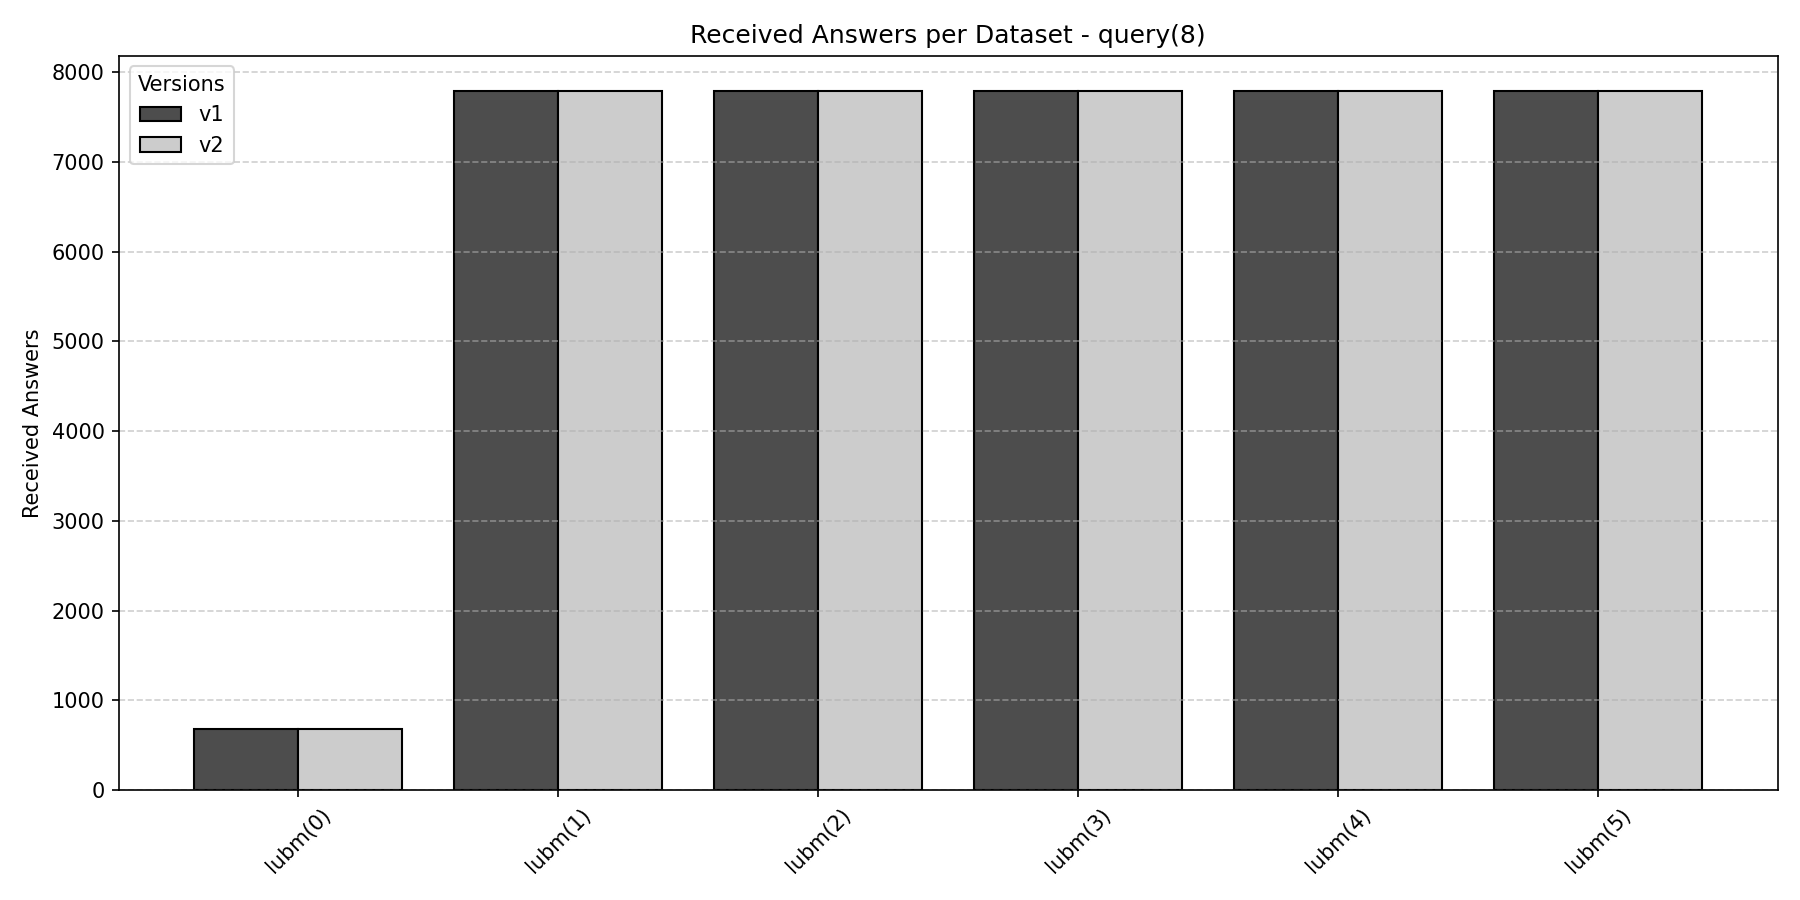
\includegraphics[width=\linewidth]{Figures/chapter5/lubm/received_answers_query8.png}
    \caption{Received answer for \gls{LUBM} query 8.}
    \label{plot-query-results-q8}
\end{figure}

\begin{figure}[H]
    \centering
    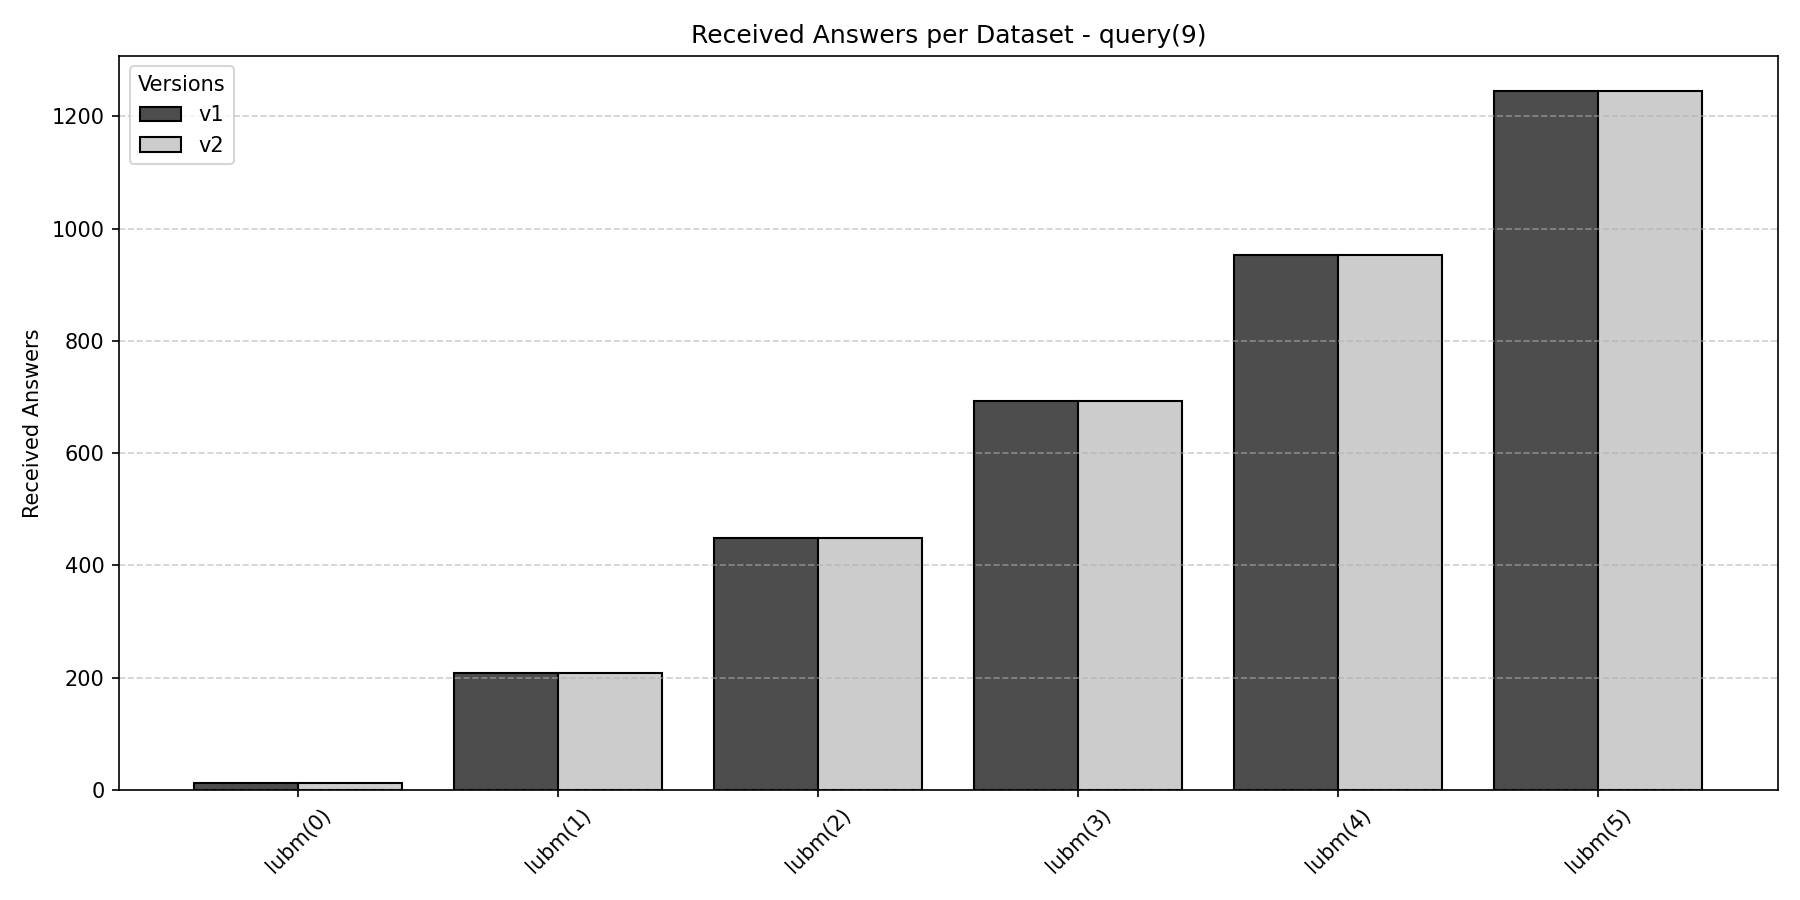
\includegraphics[width=\linewidth]{Figures/chapter5/lubm/received_answers_query9.png}
    \caption{Received answer for \gls{LUBM} query 9.}
    \label{plot-query-results-q9}
\end{figure}

\begin{figure}[H]
    \centering
    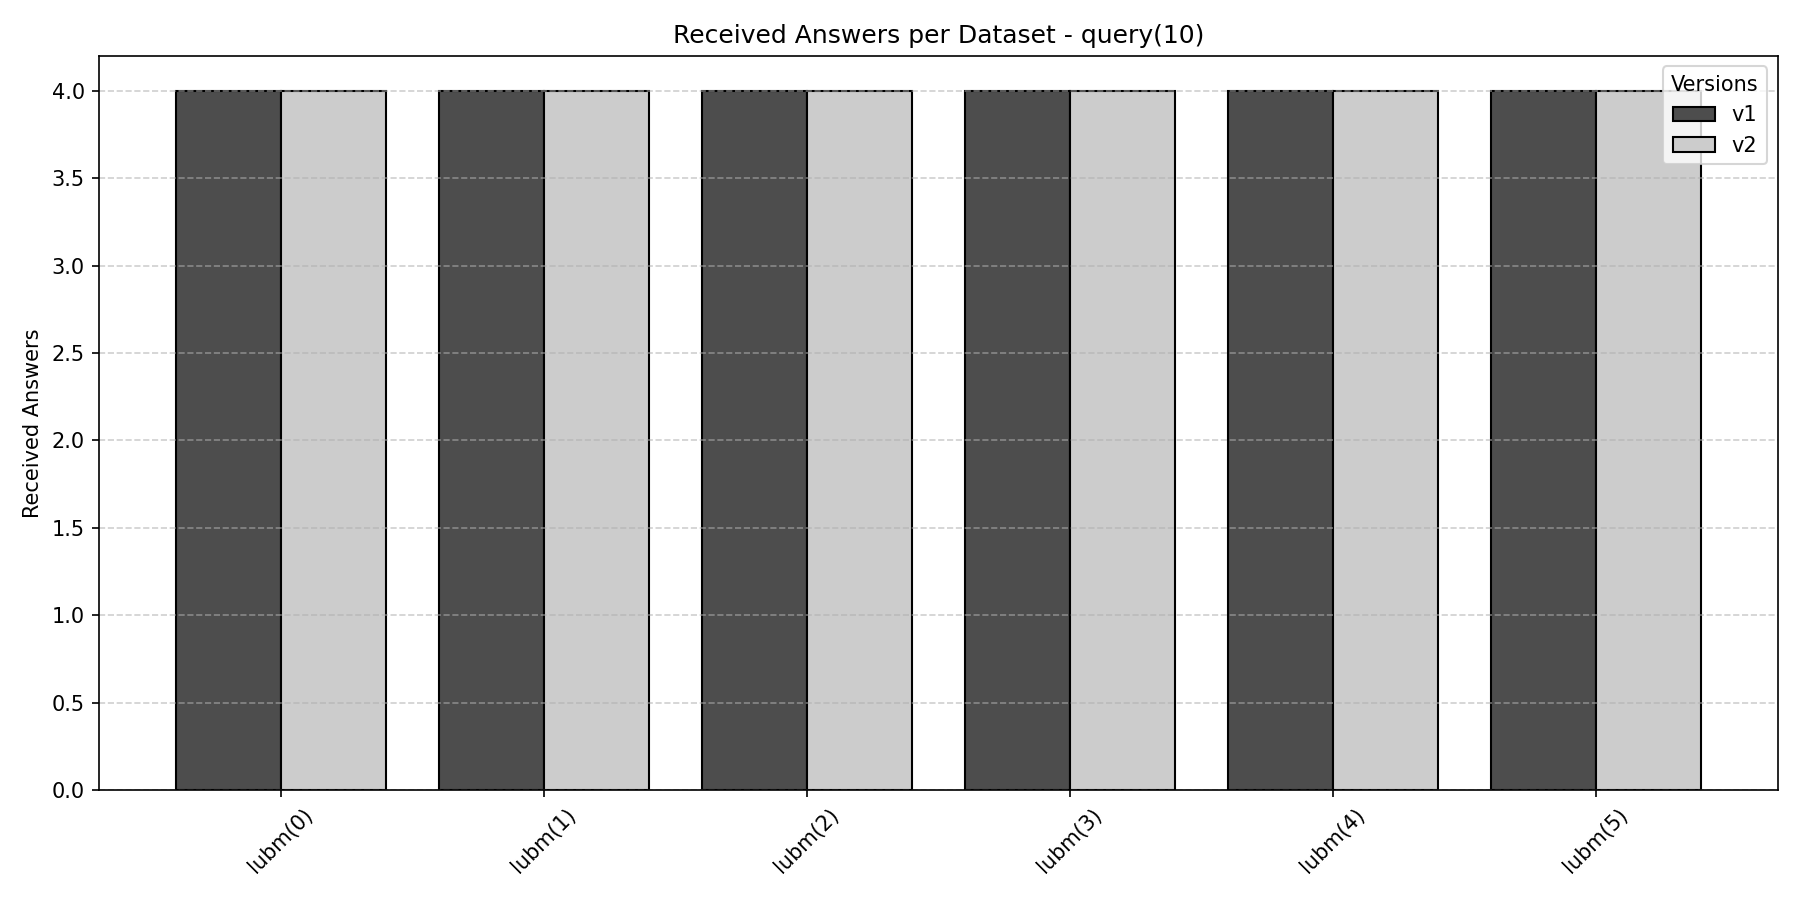
\includegraphics[width=\linewidth]{Figures/chapter5/lubm/received_answers_query10.png}
    \caption{Received answer for \gls{LUBM} query 10.}
    \label{plot-query-results-q10}
\end{figure}

\begin{figure}[H]
    \centering
    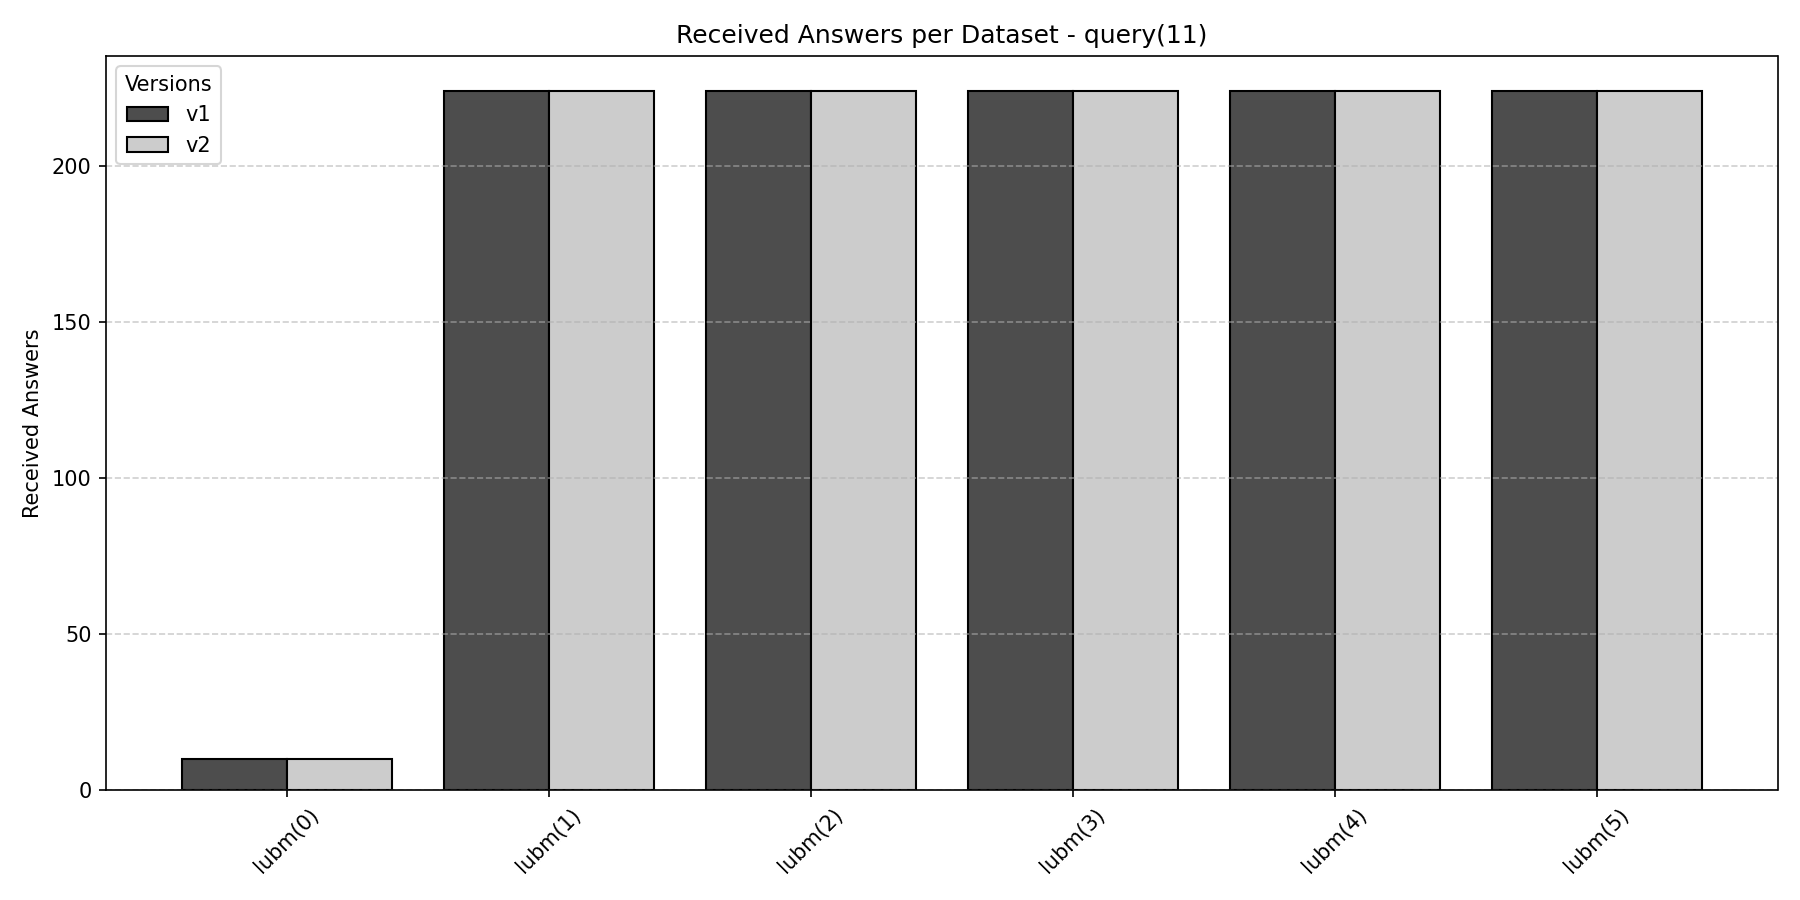
\includegraphics[width=\linewidth]{Figures/chapter5/lubm/received_answers_query11.png}
    \caption{Received answer for \gls{LUBM} query 11.}
    \label{plot-query-results-q11}
\end{figure}

\begin{figure}[H]
    \centering
    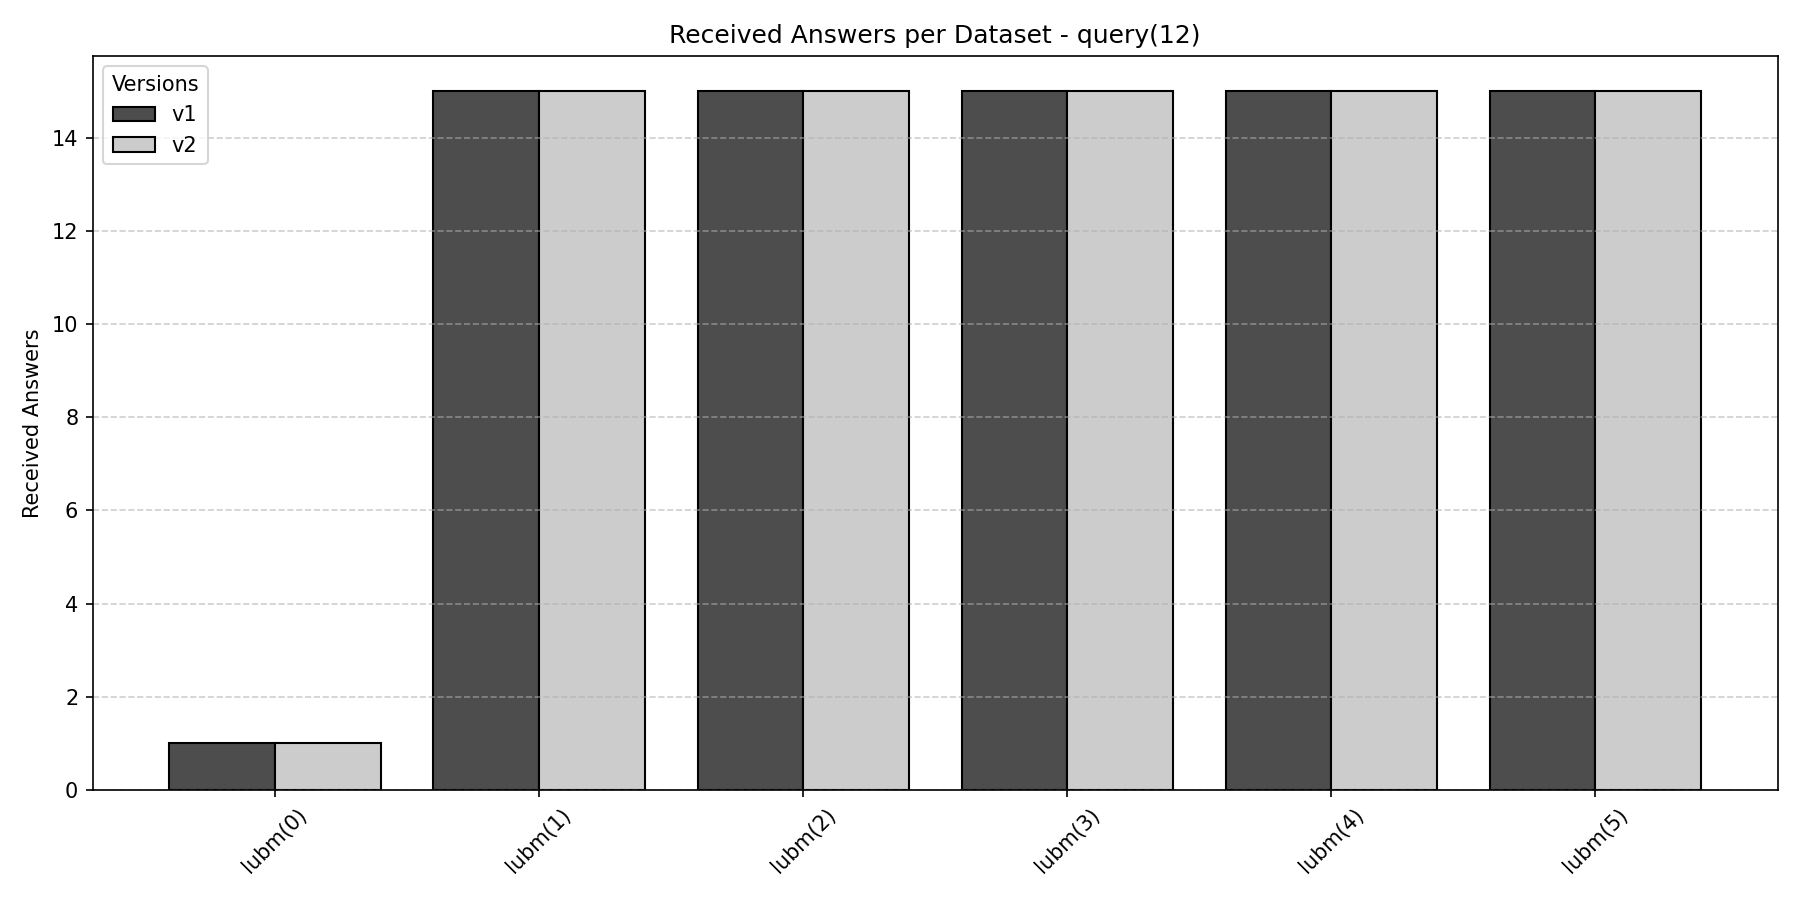
\includegraphics[width=\linewidth]{Figures/chapter5/lubm/received_answers_query12.png}
    \caption{Received answer for \gls{LUBM} query 12.}
    \label{plot-query-results-q12}
\end{figure}

\begin{figure}[H]
    \centering
    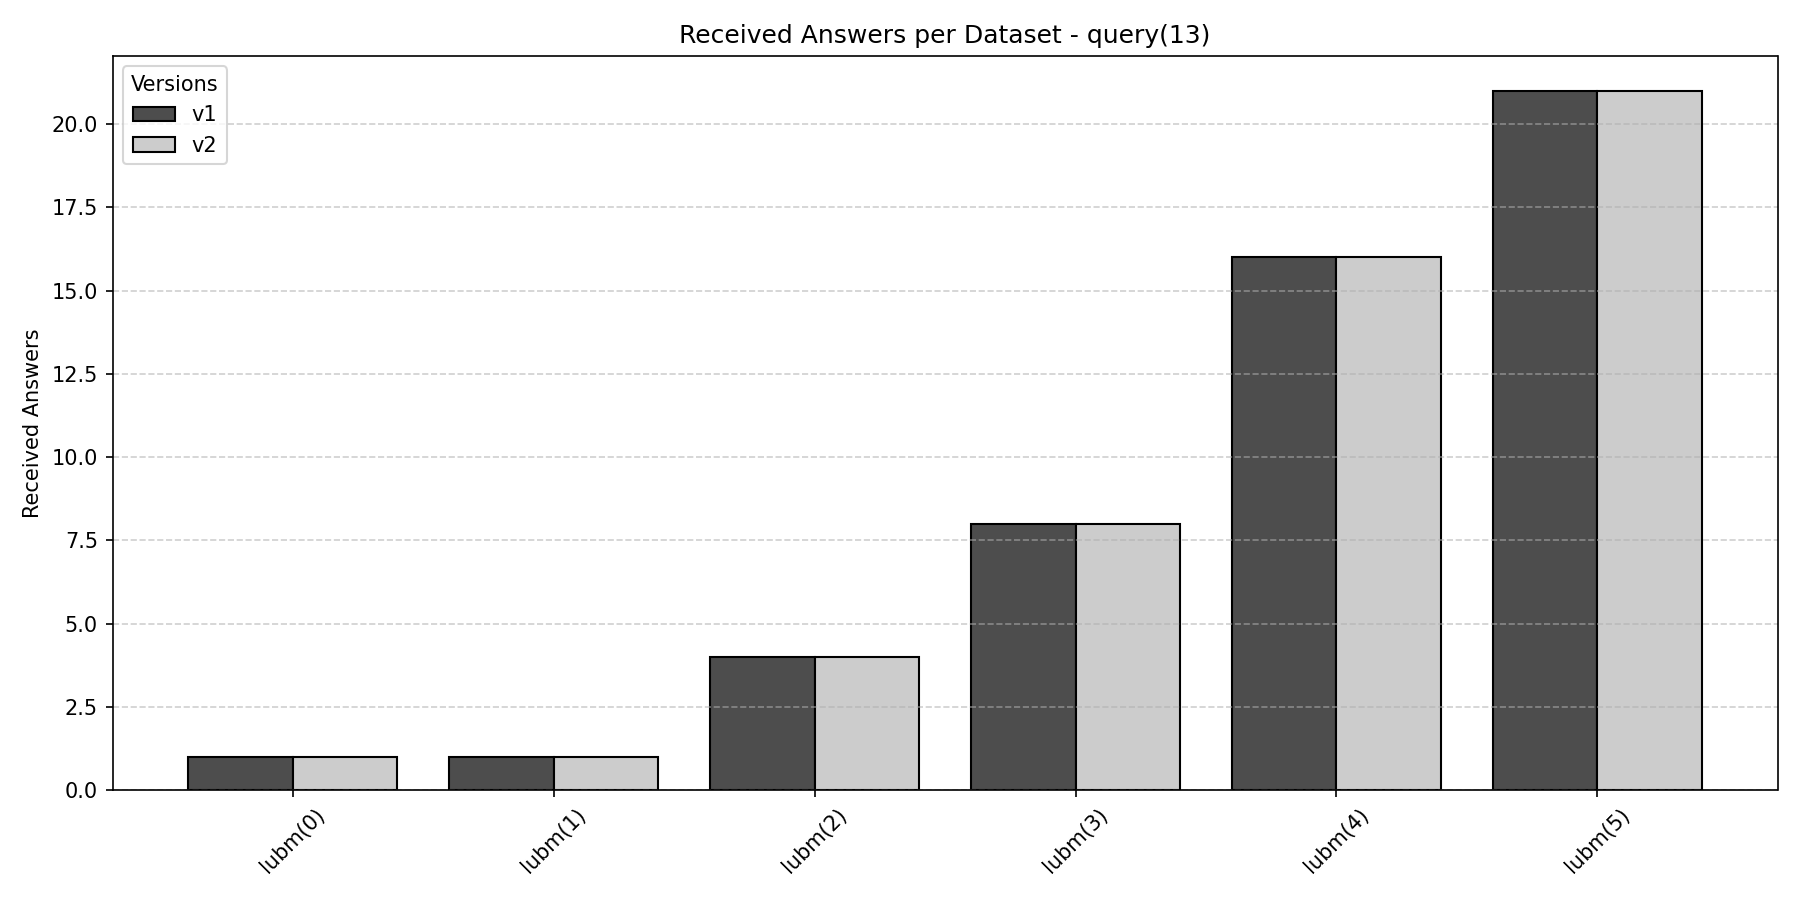
\includegraphics[width=\linewidth]{Figures/chapter5/lubm/received_answers_query13.png}
    \caption{Received answer for \gls{LUBM} query 13.}
    \label{plot-query-results-q13}
\end{figure}

\begin{figure}[H]
    \centering
    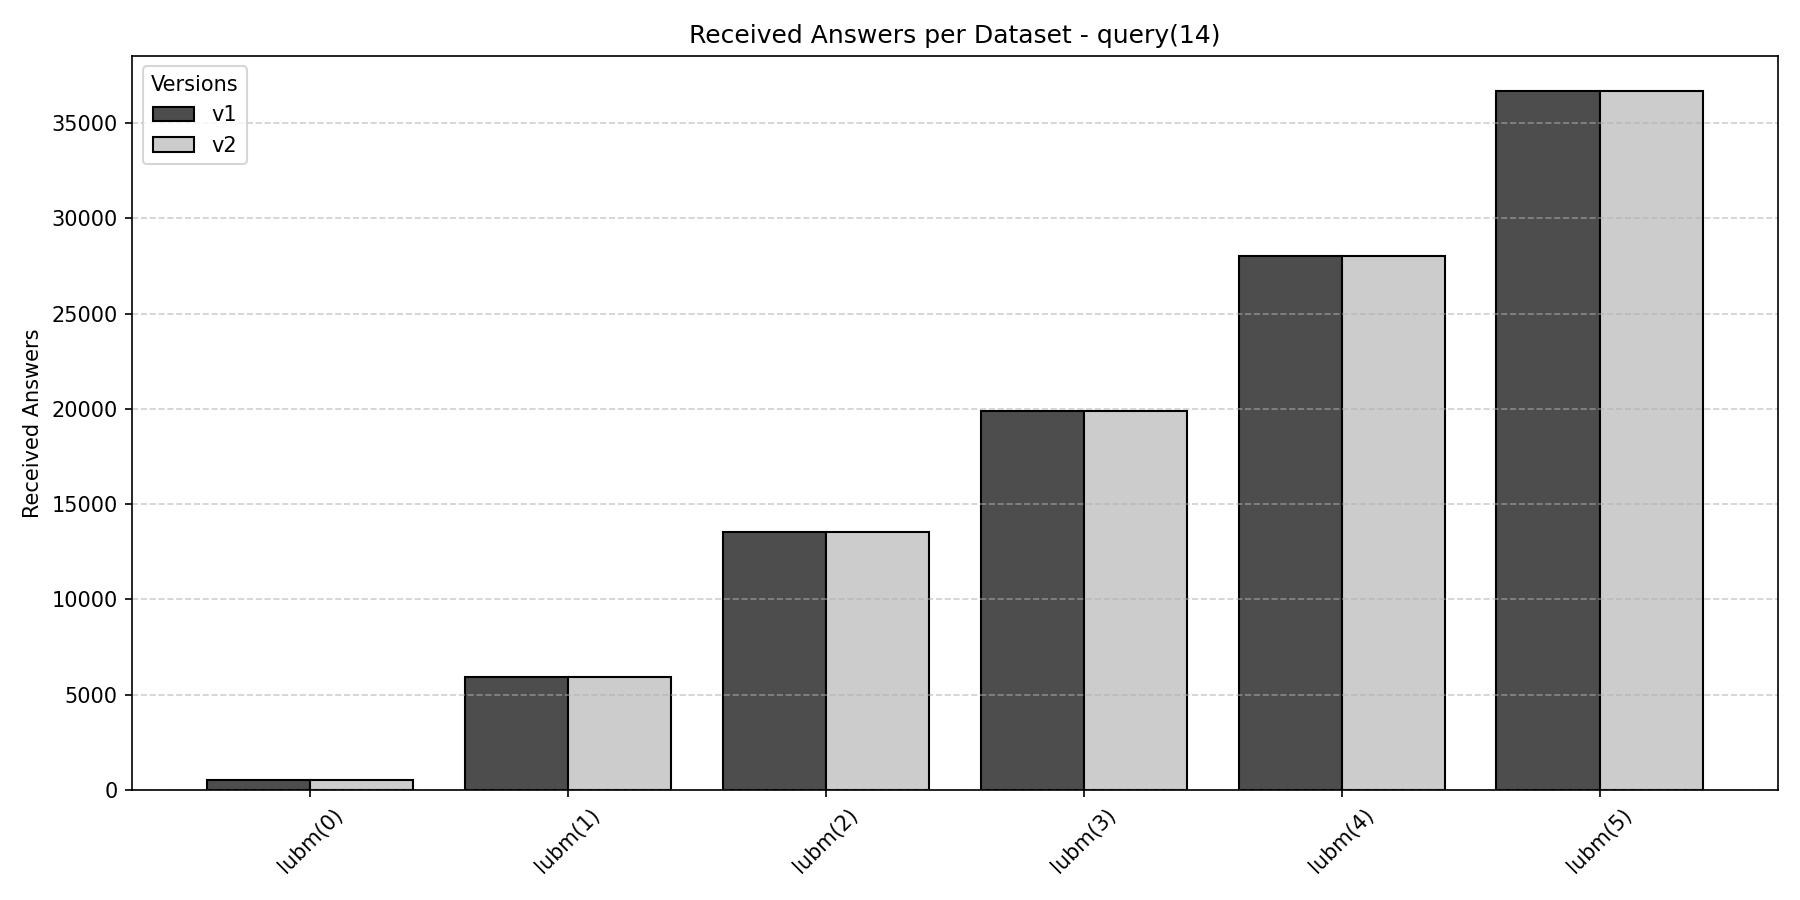
\includegraphics[width=\linewidth]{Figures/chapter5/lubm/received_answers_query14.png}
    \caption{Received answer for \gls{LUBM} query 14.}
    \label{plot-query-results-q14}
\end{figure}


